%% AI-CogWalk-NAV: projeto de pesquisa no modelo de dissertação do PPGTI/IFPB (abnTeX2)
%% Compilar com: pdflatex -> bibtex -> pdflatex -> pdflatex   (no Overleaf: compilador pdfLaTeX)
\documentclass[12pt,oneside,a4paper,chapter=TITLE,english,brazil]{abntex2}

% ---------- Dados do trabalho: altere aqui ----------
\newcommand{\proj}{AI-CogWalk-NAV}
\titulo{\proj: Previsão da Distribuição de Escolhas de Navegação de Usuários Iniciantes com Modelos de Linguagem e Princípios do Percurso Cognitivo}
\autor{Lucas Matheus Silva}
\local{João Pessoa}
\data{2026}
\orientador{A definir}
\instituicao{Instituto Federal de Educação, Ciência e Tecnologia da Paraíba}
\tipotrabalho{Projeto de Pesquisa}
% Texto da capa. Quando o trabalho virar dissertação, troque por DISSERTAÇÃO DE MESTRADO.
\newcommand{\tipocapa}{PROJETO DE PESQUISA DE MESTRADO}
\preambulo{Projeto de pesquisa apresentado ao Programa de Pós-Graduação em Tecnologia da Informação do Instituto Federal de Educação, Ciência e Tecnologia da Paraíba -- IFPB, como proposta de dissertação de mestrado.}
% -----------------------------------------------------

\usepackage[T1]{fontenc}
\usepackage[utf8]{inputenc}
\usepackage{times}
\renewcommand{\ttdefault}{lmtt}
\renewcommand{\sfdefault}{lmss}
\usepackage{indentfirst}
\usepackage{microtype}
\usepackage{graphicx}
\usepackage[table]{xcolor}
\usepackage{amsmath,amssymb}
\usepackage{booktabs}
\usepackage{tabularx}
\usepackage{multirow}
\usepackage{enumitem}
\usepackage{tikz}
\usepackage{pgfplots}
\pgfplotsset{compat=1.17}
\pgfkeys{/pgf/number format/.cd,use comma,1000 sep={.}}
\usepackage{pgfgantt}
\usepackage[most]{tcolorbox}
\usepackage{textcomp}
\usepackage{listings}
\usetikzlibrary{arrows.meta, positioning, shapes.geometric, fit, backgrounds, calc}

% Citações no padrão ABNT (autor, ano), com a página em que cada obra foi citada
\usepackage[brazilian,hyperpageref]{backref}
\usepackage[alf,abnt-emphasize=em]{abntex2cite}
\renewcommand{\backrefpagesname}{Citado na(s) página(s):~}
\renewcommand{\backref}{}
\renewcommand*{\backrefalt}[4]{%
  \ifcase #1 Nenhuma citação no texto.%
  \or Citado na página #2.%
  \else Citado #1 vezes nas páginas #2.%
  \fi}

% Aparência no estilo do modelo do PPGTI: títulos em Times negrito
\renewcommand{\ABNTEXchapterfont}{\rmfamily\bfseries}
\renewcommand{\ABNTEXchapterfontsize}{\Large}
\renewcommand{\ABNTEXsectionfontsize}{\large}
\renewcommand{\ABNTEXsubsectionfontsize}{\normalsize}
\renewcommand{\ABNTEXsubsubsectionfontsize}{\normalsize}
\setlength{\parindent}{1.25cm}
\setlength{\parskip}{0.15cm}
\setlength{\headheight}{15pt}
\setlength{\ABNTEXsignwidth}{10cm}
\setsecnumdepth{subsubsection}
\settocdepth{subsubsection}

\definecolor{blue}{RGB}{31,56,120}
\hypersetup{colorlinks=true,linkcolor=black,citecolor=black,urlcolor=blue,filecolor=black,bookmarksdepth=4}
\makeatletter
\hypersetup{pdftitle={\@title},pdfauthor={\@author},pdfsubject={\imprimirpreambulo},pdfcreator={LaTeX com abnTeX2}}
\makeatother

% Comandos do texto
\newcommand{\code}[1]{\texttt{#1}}
\def\UrlBreaks{\do\/\do-\do_}
\newcolumntype{Y}{>{\raggedright\arraybackslash}X}
\newcommand{\Ph}{P_H}
\newcommand{\Pp}{\hat{P}}
\DeclareMathOperator{\JSD}{JSD}
\newcommand{\melhor}[1]{\,$#1$}

% Caixas de situação: o que é resultado medido e o que é planejado
\newtcolorbox{real}{breakable,colback=green!4,colframe=green!45!black,boxrule=0.5pt,arc=2pt,left=5pt,right=5pt,top=3pt,bottom=3pt,
  fonttitle=\bfseries\small,title=Resultado real (executado em 13/11/2026),before upper={\setlength{\parindent}{0pt}\setlength{\parskip}{4pt}\small}}
\newtcolorbox{planejado}{breakable,colback=orange!5,colframe=orange!70!black,boxrule=0.5pt,arc=2pt,left=5pt,right=5pt,top=3pt,bottom=3pt,
  fonttitle=\bfseries\small,title=Planejado (ainda não executado),before upper={\setlength{\parindent}{0pt}\setlength{\parskip}{4pt}\small}}
\newtcolorbox{destaque}[1][]{breakable,colback=gray!5,colframe=gray!60,boxrule=0.4pt,arc=2pt,left=5pt,right=5pt,top=3pt,bottom=3pt,
  fonttitle=\bfseries\small,title=#1,before upper={\setlength{\parindent}{0pt}\setlength{\parskip}{4pt}\small}}

\lstset{basicstyle=\ttfamily\fontsize{7.5}{9.5}\selectfont,upquote=true,breaklines=true,breakindent=1.5em,frame=single,columns=fullflexible,inputencoding=utf8,extendedchars=true,
  literate={á}{{\'a}}1 {é}{{\'e}}1 {í}{{\'i}}1 {ó}{{\'o}}1 {ú}{{\'u}}1 {ã}{{\~a}}1 {õ}{{\~o}}1 {ç}{{\c{c}}}1 {â}{{\^a}}1 {ê}{{\^e}}1 {ô}{{\^o}}1 {–}{{--}}1 {—}{{---}}1 {×}{{$\times$}}1}

\setlist[itemize]{leftmargin=1.6cm,itemsep=1pt,topsep=3pt}
\setlist[enumerate]{leftmargin=1.6cm,itemsep=1pt,topsep=3pt}
\captionnamefont{\small}\captiontitlefont{\small}
\renewcommand{\arraystretch}{1.2}

% Capa no formato do modelo do PPGTI
\renewcommand{\imprimircapa}{%
  \begin{capa}%
    \centering
    
\includegraphics[width=3.3cm]{figuras/logo-ifpb.png}\par
    \vspace{0.5cm}
    {\bfseries\small
      Instituto Federal de Educação, Ciência e Tecnologia da Paraíba\par\vspace{5pt}
      Campus João Pessoa\par\vspace{5pt}
      Programa de Pós-Graduação em Tecnologia da Informação\par\vspace{5pt}
      Nível Mestrado Profissional\par}
    \vspace{2.6cm}
    {\bfseries\MakeUppercase{\imprimirautor}\par}
    \vspace{0.8cm}
    {\bfseries\large\MakeUppercase{\imprimirtitulo}\par}
    \vspace{2.2cm}
    {\bfseries\footnotesize\tipocapa\par}
    \vfill
    {\bfseries\MakeUppercase{\imprimirlocal}\par\imprimirdata\par}
    \vspace*{0.5cm}
  \end{capa}}

% Nome da lista de figuras como no modelo do PPGTI
\addto\captionsbrazil{\renewcommand{\listfigurename}{Lista de Figuras}}
% Âncoras únicas para figuras e tabelas (a numeração é contínua no documento)
\AtBeginDocument{\renewcommand{\theHfigure}{fig.\arabic{figure}}\renewcommand{\theHtable}{tab.\arabic{table}}}

\makeindex

\begin{document}
\selectlanguage{brazil}
\frenchspacing

% =====================================================================
% ELEMENTOS PRÉ-TEXTUAIS
% =====================================================================
\pretextual
\hypersetup{pageanchor=false}
\imprimircapa
\imprimirfolhaderosto

\setlength{\absparsep}{12pt}
\begin{resumo}
Quando iniciantes procuram uma informação num portal institucional, parte deles dá um primeiro passo errado, e a proporção depende dos rótulos, do leiaute e da tarefa. Este trabalho apresenta o \textit{\proj}, um método e um protótipo que preveem, antes de observar qualquer usuário, a \emph{distribuição} das primeiras escolhas de navegação de iniciantes, $P_H(a \mid s, t)$, a partir da tarefa e das opções visíveis numa tela, e a comparam com escolhas observadas em pessoas. O estudo investiga se a incorporação controlada de princípios do percurso cognitivo aplicáveis à primeira escolha (objetivo, visibilidade e associação do rótulo) e de estratégias de amostragem modifica a fidelidade das distribuições previstas por modelos de linguagem de grande escala (LLMs), em comparação com uma \textit{baseline} semântica convencional. Uma condição de controle separa o efeito das perguntas do percurso cognitivo do efeito de apenas deliberar sobre cada opção. O protocolo usa previsões congeladas, um \textit{benchmark} público com 1.796 primeiros cliques em seis variantes de apresentação, validação cruzada em duas partes por tarefa e a divergência de Jensen--Shannon como métrica principal, com intervalos por \textit{bootstrap} de tarefas, testes exatos de troca de sinal e correção de Holm. O que já foi executado está relatado como resultado: a implementação foi conferida de forma independente; a \textit{baseline} semântica (B0) ficou abaixo do acaso em 8 de 10 tarefas, com diferença média de $-0{,}087$ na divergência, mas a significância desse resultado depende de como a sua temperatura é escolhida; a variação das escolhas humanas entre as seis apresentações não se distingue do ruído de amostras de 30 pessoas; e um piloto de quatro estados com GPT-4.1 e Claude Opus~5.5 verificou prompts, armazenamento, isolamento das entradas e custos. O experimento completo com LLMs e o piloto prospectivo no portal do IFPB estão planejados e descritos passo a passo.

\textbf{Palavras-chave}: percurso cognitivo; primeiro clique; modelos de linguagem de grande escala; arquitetura da informação; usabilidade; participantes simulados.
\end{resumo}

\begin{resumo}[Abstract]
\begin{otherlanguage*}{english}
When novices look for information in an institutional website, some of them take a wrong first step, and how many do so depends on the labels, the layout and the task. This work presents \textit{\proj}, a method and a prototype that predict, before any user is observed, the \emph{distribution} of first navigation choices of novices, $P_H(a \mid s, t)$, from the task and the options visible on one screen, and compare it with choices observed in people. The study asks whether the controlled incorporation of cognitive walkthrough principles applicable to the first choice (goal, visibility and label association) and of sampling strategies changes the fidelity of distributions predicted by large language models (LLMs), compared with a conventional semantic baseline. A control condition separates the effect of the walkthrough questions from that of simply deliberating about each option. The protocol uses frozen predictions, a public benchmark with 1,796 first clicks in six presentation variants, two-fold cross-validation by task and the Jensen--Shannon divergence as primary metric, with task-level bootstrap intervals, exact sign-flip tests and Holm correction. What has already been executed is reported as results: the implementation was verified independently; the semantic baseline (B0) stayed below chance in 8 of 10 tasks, with a mean difference of $-0.087$ in divergence, but the significance of this result depends on how its temperature is chosen; the variation of human choices across the six presentations cannot be distinguished from the noise of samples of 30 people; and a four-state pilot with GPT-4.1 and Claude Opus~5.5 checked prompts, storage, input isolation and costs. The full LLM experiment and the prospective pilot in the IFPB portal are planned and described step by step.

\textbf{Keywords}: cognitive walkthrough; first click; large language models; information architecture; usability; simulated participants.
\end{otherlanguage*}
\end{resumo}

\pdfbookmark[0]{\listfigurename}{lof}
\listoffigures*
\cleardoublepage
\pdfbookmark[0]{\listtablename}{lot}
\listoftables*
\cleardoublepage

\begin{siglas}
  \item[API] \textit{Application Programming Interface}
  \item[B0] \textit{Baseline} semântica sem LLM: semelhança entre a tarefa e cada rótulo
  \item[B1] LLM que declara, numa única chamada, a distribuição de escolhas de iniciantes
  \item[B1-CW] B1 com as perguntas Q1 a Q3 do percurso cognitivo respondidas para cada opção
  \item[B1-R] Controle do B1-CW: análise livre de cada opção, sem as perguntas do percurso cognitivo
  \item[B1-S] LLM como participante simulado: $N$ chamadas independentes, uma escolha por chamada
  \item[B1-CW-S] B1-S em que cada participante simulado passa por Q1 a Q3 antes de escolher
  \item[B2] Sistema multiagente, previsto para uma fase posterior
  \item[CEP] Comitê de Ética em Pesquisa
  \item[CW] \textit{Cognitive Walkthrough} (percurso cognitivo)
  \item[CWW] \textit{Cognitive Walkthrough for the Web}
  \item[DEV] Metade de desenvolvimento do \textit{benchmark}: tarefas pares
  \item[DOM] \textit{Document Object Model}
  \item[IC] Intervalo de confiança
  \item[IFPB] Instituto Federal de Educação, Ciência e Tecnologia da Paraíba
  \item[IHC] Interação Humano-Computador
  \item[JSD] Divergência de Jensen--Shannon
  \item[LGPD] Lei Geral de Proteção de Dados Pessoais
  \item[LLM] \textit{Large Language Model} (modelo de linguagem de grande escala)
  \item[PPGTI] Programa de Pós-Graduação em Tecnologia da Informação
  \item[Q1 a Q4] As quatro perguntas do percurso cognitivo
  \item[QP] Questão de pesquisa
  \item[TEST] Metade de teste do \textit{benchmark}: tarefas ímpares
  \item[TP, TC, TO] Variantes do \textit{benchmark} em texto (\textit{tree testing})
  \item[UNIFORM] Referência que dá a mesma probabilidade a todas as opções (o acaso)
  \item[UX] \textit{User Experience} (experiência do usuário)
  \item[WTC, WTCI, WM] Variantes visuais do \textit{benchmark}: \textit{desktop}, \textit{desktop} com elementos intrusivos e celular
\end{siglas}

\pdfbookmark[0]{\contentsname}{toc}
\tableofcontents*
\cleardoublepage

% =====================================================================
% ELEMENTOS TEXTUAIS
% =====================================================================
\textual
\hypersetup{pageanchor=true}
\sloppy

% =====================================================================
\chapter{Introdução}
\label{cap:intro}
% =====================================================================

Este capítulo apresenta o problema de prever, antes de observar qualquer pessoa, para onde iniciantes vão no primeiro clique de uma tarefa de navegação. A partir dessa contextualização, formula a hipótese central e as questões de pesquisa. Em seguida, são apresentados os objetivos, a justificativa, uma visão geral da metodologia, as contribuições pretendidas, a situação atual do trabalho e a organização do documento.

\section{Contextualização e Problema de Pesquisa}
\label{sec:contexto}

Portais institucionais concentram serviços que estudantes e cidadãos precisam encontrar sozinhos: editais, declarações, calendários, processos seletivos. Quem os usa pela primeira vez não conhece a estrutura administrativa da instituição e decide pelo que vê na tela: rótulos, posição, destaque. Uma escolha errada no primeiro nível costuma custar caro, porque a pessoa precisa perceber o erro, voltar e tentar outro caminho, e parte desiste. \citeonline{bailey2009firstclick} relatam que participantes cujo primeiro clique foi correto completaram a tarefa com chance de 0,87, contra 0,46 entre os que erraram o primeiro clique. O artigo não informa o tamanho das amostras, de modo que os valores servem de indicação, e não de estimativa precisa.

Testes com usuários revelam esses desvios, mas são caros e chegam tarde. Métodos de inspeção, como o percurso cognitivo (\textit{cognitive walkthrough}, CW), antecipam dificuldades sem usuários. Neles, o avaliador pergunta, a cada passo, se o iniciante vai querer fazer a ação certa, se vai perceber o controle, se vai associá-lo ao objetivo e se vai entender o retorno \cite{polson1992cw,wharton1994cw}. Modelos de \textit{information scent} vão além e preveem quais links serão escolhidos a partir da semelhança entre o objetivo e os rótulos \cite{pirolli1999foraging,blackmon2002cww,fu2007snifact}.

Modelos de linguagem de grande escala (LLMs) multimodais trouxeram uma nova possibilidade: ler a tela como uma pessoa lê e estimar o que um iniciante faria. Trabalhos recentes já usam LLMs para conduzir percursos cognitivos \cite{bisante2024cwgpt,zhong2025syntheticcw}, simular usuários \cite{lu2025uxagent,tan2026avenirux,chowdhury2026amuser} e prever o primeiro clique de participantes \cite{kuric2026wwgc,hu2025uitransition}. O resultado mais próximo deste trabalho, \textit{What Would GPT Click} \cite{kuric2026wwgc}, mostra o limite atual. O LLM acerta a opção mais escolhida em 71\% das tarefas, mas a distribuição prevista difere de forma significativa da humana em 53\% delas. A previsão é concentrada demais, com menos opções e menos dispersão do que as escolhas de pessoas reais.

Esse é o ponto de partida do \proj. Não basta acertar a opção mais provável: num portal, o que importa ao projetista é \emph{quantos} iniciantes vão para cada lado, e em particular quantos vão para o lado errado. O objeto de previsão deste trabalho é, portanto, a distribuição das primeiras escolhas,
\begin{equation}
\Ph(a \mid s, t), \qquad a \in A(s),
\end{equation}
em que $s$ é o estado da interface (a tela), $t$ é a tarefa e $A(s)$ é o conjunto de opções visíveis. O preditor recebe apenas o que o iniciante tem no momento da decisão (a tarefa, a tela e as opções) e nunca o caminho correto, o destino ou dados humanos do estado avaliado.

\subsection{Um exemplo real}

A Figura~\ref{fig:exemplo} mostra um estado do \textit{benchmark} usado neste trabalho. A tarefa diz que o \textit{laptop} da pessoa parou de funcionar e pergunta onde ela procuraria orientação sobre a marca e o modelo de um novo. O menu tem oito categorias. Das 30 pessoas, 12 clicaram primeiro em Lifestyle, 7 em Hobbies, 5 em Entertainment, 4 em Science e 2 em Trending. Nenhuma opção reuniu a maioria. Um método que respondesse apenas ``Lifestyle'' acertaria a opção mais escolhida e esconderia que 60\% das pessoas foram para outro lugar. É essa repartição que o \proj{} tenta prever.

\begin{figure}[htb]
\centering
\caption{Um estado real do \textit{benchmark} (variante TP, tarefa 8): primeira escolha de 30 pessoas que procuravam orientação para comprar um \textit{laptop}. A opção mais escolhida reúne só 40\% das pessoas.}
\label{fig:exemplo}
\begin{tikzpicture}
\begin{axis}[
  ybar, bar width=14pt, width=0.95\textwidth, height=4.6cm, ymin=0, ymax=15, enlarge x limits=0.08,
  ylabel={pessoas (de 30)},
  symbolic x coords={Trending,Entertainment,Hobbies,Culture,Science,Society,Lifestyle,About us}, xtick=data,
  x tick label style={font=\scriptsize}, label style={font=\footnotesize}, y tick label style={font=\footnotesize},
  nodes near coords, nodes near coords style={font=\footnotesize}
]
\addplot[fill=gray!55] coordinates {(Trending,2) (Entertainment,5) (Hobbies,7) (Culture,0) (Science,4) (Society,0) (Lifestyle,12) (About us,0)};
\end{axis}
\end{tikzpicture}
\legend{Fonte: elaborada pelo autor, com dados de \citeonline{kuric2025dataset}.}
\end{figure}

\subsection{Hipótese central e questões de pesquisa}

\begin{destaque}[Hipótese central]
A incorporação controlada de princípios cognitivos e de estratégias de amostragem modifica a fidelidade das distribuições de escolhas previstas por LLMs em relação às escolhas humanas de primeiro clique, quando comparada a uma \textit{baseline} semântica convencional.
\end{destaque}

A hipótese fala em primeiro clique porque é isso que o \textit{benchmark} mede. Trajetórias completas (cliques seguintes, recuos e abandono) ficam para uma fase posterior. A hipótese é decomposta em quatro questões de pesquisa:

\begin{itemize}
\item \textbf{QP1 (fidelidade).} Quão próxima da distribuição humana fica a distribuição prevista por um LLM (condição B1), comparada à \textit{baseline} semântica (B0) e à referência uniforme?
\item \textbf{QP2 (princípios cognitivos).} Pedir ao LLM que aplique as perguntas do CW pertinentes à primeira escolha (Q1 objetivo, Q2 visibilidade, Q3 associação) altera a fidelidade (B1-CW contra B1)? E o efeito vem das perguntas do CW ou apenas de deliberar sobre cada opção (B1-CW contra o controle B1-R)?
\item \textbf{QP3 (amostragem).} Estimar a distribuição por participantes simulados independentes (B1-S) produz distribuições mais ou menos fiéis e mais ou menos dispersas do que pedir a distribuição numa única chamada (B1)?
\item \textbf{QP4 (modalidade e apresentação).} Os efeitos mudam entre menus apresentados como texto (\textit{tree testing}) e protótipos visuais, em \textit{desktop} e celular?
\end{itemize}

\section{Objetivos}
\label{sec:objetivos}

\subsection{Objetivo Geral}

Investigar se LLMs multimodais preveem com fidelidade a distribuição das primeiras escolhas de navegação de usuários iniciantes e se a incorporação controlada de princípios do percurso cognitivo e de estratégias de amostragem altera essa fidelidade.

\subsection{Objetivos Específicos}

\begin{enumerate}
\item Formalizar a previsão do primeiro clique como previsão de uma distribuição e definir as métricas e as referências para avaliá-la (Seções~\ref{sec:formal} e~\ref{sec:metricas}).
\item Construir e validar um protótipo que isole as entradas do preditor, congele as previsões e torne as rodadas reprodutíveis (Seções~\ref{sec:arquitetura} e~\ref{sec:validacao}).
\item Estabelecer as referências de comparação: o acaso (UNIFORM), uma \textit{baseline} semântica sem LLM (B0), o piso amostral e a referência humana entre variantes (QP1).
\item Medir o efeito das perguntas Q1 a Q3 sobre a distribuição prevista, separando-o do efeito de apenas deliberar sobre cada opção (QP2).
\item Comparar a distribuição declarada numa única chamada com a obtida de participantes simulados independentes (QP3).
\item Verificar se os efeitos mudam entre apresentações em texto e apresentações visuais (QP4).
\item Aplicar o método de forma prospectiva a um portal institucional em português, com as previsões congeladas antes da coleta com pessoas (Seção~\ref{sec:ifpb}).
\end{enumerate}

\section{Justificativa}
\label{sec:justificativa}

\textbf{Relevância prática.} Em portais institucionais, quem chega pela primeira vez é justamente quem mais precisa do serviço: o ingressante procurando uma declaração, o candidato procurando um edital. Esses usuários não conhecem os nomes internos dos setores, e uma escolha errada no primeiro nível os leva a páginas que não respondem à pergunta. Saber, antes de publicar, que (por exemplo) 40\% dos iniciantes devem ir para ``Pesquisa'' em vez de ``Editais'' permite renomear, reagrupar ou duplicar um link com custo baixo.

\textbf{Por que uma distribuição, e não um único clique.} Iniciantes diferentes decidem de forma diferente diante da mesma tela. No \textit{benchmark} usado aqui, a opção mais escolhida reúne, em média, só 58\% das pessoas, e em 28\% dos estados nenhuma opção chega à metade (Seção~\ref{sec:humanos}). Um preditor que acerta a opção mais escolhida, mas ignora os 40\% que vão para outro lado, esconde exatamente o problema que interessa ao projetista. Os próprios dados mostram quanto isso pesa: uma ``previsão'' que colocasse toda a probabilidade na opção mais escolhida de cada estado, usando os dados humanos, acertaria o primeiro lugar em todos os estados e ainda assim ficaria com divergência de 0,259, pouco melhor que a de uma \textit{baseline} simples (Seção~\ref{sec:humanos}). Prever a distribuição também evita exigir do modelo que adivinhe a escolha de uma pessoa específica. \citeonline{dillion2023replace} observam que modelos de linguagem aproximam bem a resposta média das pessoas, mas não a variação entre elas, e é essa variação que o \proj{} tenta prever.

\textbf{Por que testar princípios cognitivos.} O percurso cognitivo foi desenhado para iniciantes que aprendem explorando \cite{polson1992cw,wharton1994cw}. Suas perguntas descrevem o mecanismo da primeira escolha: a pessoa forma uma intenção (Q1), procura o controle (Q2) e julga se o rótulo combina com o que tem em mente (Q3). Se pedir ao LLM que raciocine por essas perguntas aproxima a distribuição prevista da humana, há um ganho metodológico concreto. Se afasta, por exemplo tornando o modelo mais ``confiante'', isso também é um resultado útil, porque mostra que uma estrutura de raciocínio de especialista não equivale ao comportamento de um iniciante. Há um antecedente nas duas direções: \citeonline{zhong2025syntheticcw} relatam que LLMs completam mais tarefas e seguem caminhos mais eficientes do que pessoas, mas que, com prompts adicionais, passam a prever os pontos em que as pessoas falham.

\textbf{Por que testar amostragem.} LLMs tendem a responder como ``super-usuários'': escolhem o caminho mais racional e variam pouco \cite{kuric2026wwgc,zhong2025syntheticcw}. O padrão já tinha sido descrito fora da área de Interação Humano-Computador (IHC). \citeonline{aher2023turing} chamam de distorção de hiperacurácia a tendência de alguns modelos a responder com mais acerto do que as pessoas que deveriam simular, e \citeonline{bisbee2024synthetic} mostram que respostas sintéticas têm menos variação do que as de uma pesquisa real. Há duas formas naturais de obter uma distribuição: pedir a distribuição diretamente ou simular participantes independentes e contar as escolhas. Em pesquisas de opinião, \citeonline{meister2025distributional} observaram que modelos de linguagem descrevem a distribuição de respostas de um grupo com mais acurácia do que a reproduzem quando geram uma sequência de respostas amostradas, e \citeonline{jang2026cannotsample} relatam resultado semelhante com chamadas independentes. Não se sabe se isso vale para o primeiro clique, em que a resposta depende também da tela, e a escolha entre as duas formas afeta o custo e a dispersão.

\textbf{Por que um \textit{benchmark} público antes do portal.} Avaliar previsões exige dados humanos. O conjunto de \citeonline{kuric2025ia} é público, tem 30 pessoas por estado e mostra a \emph{mesma} arquitetura de informação em seis apresentações (três de \textit{tree testing}, em texto, e três protótipos visuais). Isso permite desenvolver e validar o método sem coleta própria e sem submissão ao comitê de ética nesta fase. O portal do IFPB entra depois, como piloto prospectivo, com as previsões congeladas antes da coleta.

\section{Visão Geral da Metodologia}
\label{sec:visaogeral}

A pesquisa é empírica e quantitativa. Ela repete sempre o mesmo ciclo, resumido na Figura~\ref{fig:visao}. (1) Um \textbf{estado} é montado a partir de uma tarefa e de uma tela, com as opções visíveis. (2) Cada \textbf{condição} experimental recebe só essa entrada e devolve uma distribuição de probabilidade sobre as opções. (3) A previsão é \textbf{congelada} com um \textit{hash}. (4) Só então ela é \textbf{comparada} com as primeiras escolhas de 30 pessoas no mesmo estado. (5) As diferenças entre condições são \textbf{analisadas por tarefa}.

\begin{figure}[htb]
\centering
\caption{Visão geral do método. Os dados humanos só são usados depois de a previsão estar congelada.}
\label{fig:visao}
\begin{tikzpicture}[
  font=\scriptsize, x=0.955cm,
  stepbox/.style={draw, rounded corners=2pt, align=center, minimum height=1.25cm, text width=2.55cm, inner sep=2pt},
  arr/.style={-{Stealth[length=2mm]}, thick}
]
\node[stepbox, fill=blue!6]   (a) at (0,0)    {\textbf{1. Estado}\\tarefa + tela +\\opções visíveis};
\node[stepbox, fill=orange!8] (b) at (3.1,0)  {\textbf{2. Condição}\\UNIFORM, B0, B1,\\B1-CW, B1-R, B1-S};
\node[stepbox, fill=green!6]  (c) at (6.2,0)  {\textbf{3. Previsão}\\distribuição $\Pp$\\congelada com \textit{hash}};
\node[stepbox, fill=gray!10]  (d) at (9.3,0)  {\textbf{4. Comparação}\\com as escolhas de\\30 pessoas (JSD)};
\node[stepbox, fill=green!6]  (e) at (12.4,0) {\textbf{5. Análise}\\diferenças pareadas\\por tarefa};
\draw[arr] (a) -- (b); \draw[arr] (b) -- (c); \draw[arr] (c) -- (d); \draw[arr] (d) -- (e);
\node[font=\tiny, below=0.1cm of b, align=center, text width=2.9cm] {não recebe a rota,\\o destino nem dados humanos};
\node[font=\tiny, below=0.1cm of d, align=center, text width=2.9cm] {os dados humanos só\\entram a partir daqui};
\end{tikzpicture}
\legend{Fonte: elaborada pelo autor.}
\end{figure}

O percurso da pesquisa tem três etapas. A primeira, já concluída, construiu e validou o protótipo, mediu as referências que não usam LLM (UNIFORM e B0) e fez um piloto pequeno com dois LLMs, para verificar o funcionamento e o custo. A segunda é o experimento completo no \textit{benchmark} público: as condições com LLM são executadas uma única vez, com parâmetros congelados, e comparadas pela divergência de Jensen--Shannon (JSD) entre a distribuição prevista e a humana. A terceira é um piloto prospectivo no portal do IFPB, em que as previsões são registradas antes de qualquer coleta com pessoas. O Capítulo~\ref{cap:metodologia} detalha os dados, as condições, as hipóteses e a análise.

\section{Contribuições}
\label{sec:contribuicoes}

As contribuições pretendidas deste trabalho são:

\begin{enumerate}
\item uma \textbf{formulação do problema como previsão de distribuição}, com métricas de fidelidade (JSD), cobertura das escolhas humanas, omissões, dispersão e regras de pontuação próprias, além de um piso amostral e de uma referência humana entre variantes que mostram até onde um preditor pode chegar;
\item uma \textbf{ablação controlada dos princípios do percurso cognitivo}, separada do efeito da amostragem e do efeito de deliberar mais (condição de controle B1-R), em dois fornecedores de LLM e com os mesmos dados;
\item um \textbf{protocolo de previsões congeladas}, em que as previsões são registradas, com \textit{hash}, antes de serem comparadas com dados humanos e, no piloto institucional, antes da coleta com pessoas;
\item um \textbf{protótipo aberto e reprodutível}, que importa o \textit{benchmark}, renderiza as telas, isola as entradas do preditor, executa as condições, calcula as métricas e exporta tudo, sobre dados públicos.
\end{enumerate}

\begin{destaque}[O que este trabalho não afirma]
Não é o primeiro a usar LLMs para prever o primeiro clique \cite{kuric2026wwgc}, nem o primeiro a combinar LLM e percurso cognitivo \cite{bisante2024cwgpt,zhong2025syntheticcw}, nem o primeiro a prever problemas de navegação antes de observar usuários \cite{blackmon2002cww,blackmon2005autocww,teo2012cogtoolexplorer}. A contribuição buscada é a medição controlada do efeito de princípios cognitivos e de amostragem sobre a \emph{distribuição} prevista, com isolamento de entradas, previsões congeladas e dados públicos.
\end{destaque}

\section{Situação Atual do Trabalho e Convenções}
\label{sec:situacao}

Este documento é, ao mesmo tempo, o projeto de pesquisa e o registro do que já foi construído e medido. Para que nenhum número planejado seja confundido com um resultado, o texto usa duas caixas:

\begin{real}
Conteúdo verde: medido no protótipo, com dados reais, e reprodutível pelos comandos do Apêndice~\ref{ap:repro}.
\end{real}

\begin{planejado}
Conteúdo laranja: desenho do que ainda será feito. Não contém resultados. As rodadas completas com LLMs dependem de aprovação do orçamento.
\end{planejado}

A Tabela~\ref{tab:roteiro} resume o que cada capítulo responde e em que situação está o seu conteúdo. As siglas das condições experimentais (UNIFORM, B0, B1, B1-CW, B1-R, B1-S) e das variantes do \textit{benchmark} (TP, TC, TO, WTC, WTCI, WM) aparecem em todo o texto e estão reunidas na Lista de Abreviaturas e Siglas.

\begin{table}[htb]
\centering
\caption{Roteiro do documento e situação de cada parte.}
\label{tab:roteiro}
\footnotesize
\begin{tabularx}{\textwidth}{@{}p{4.2cm}Yp{3.3cm}@{}}
\toprule
\textbf{Capítulo} & \textbf{Pergunta que responde} & \textbf{Situação} \\
\midrule
\ref{cap:intro}. Introdução & Qual é o problema, o que se pergunta e o que se pretende entregar? & -- \\
\ref{cap:fundamentacao}. Fundamentação Teórica & Que conceitos sustentam o método? & -- \\
\ref{cap:relacionados}. Trabalhos Relacionados & O que já se sabe e o que ainda falta saber? & -- \\
\ref{cap:metodologia}. Metodologia & O que se prevê, como se mede, quais são os dados, as condições, as hipóteses e a análise? & Definida; protótipo construído; passos 1 a 9 feitos \\
\ref{cap:resultados}. Resultados Preliminares e Discussão & O protótipo mede o que diz medir? O que já foi medido? & Real \\
\ref{cap:conclusao}. Conclusão e Próximas Etapas & O que falta rodar, onde, quando e a que custo? & Planejado \\
\bottomrule
\end{tabularx}
\end{table}

\section{Estrutura do Documento}

O restante do documento está organizado da seguinte forma. O Capítulo~\ref{cap:fundamentacao} apresenta os conceitos usados: o percurso cognitivo, a teoria de \textit{information scent}, os testes de árvore e de primeiro clique, o uso de LLMs como participantes simulados, as formas de obter uma distribuição de um LLM e a avaliação de previsões probabilísticas. O Capítulo~\ref{cap:relacionados} discute os trabalhos mais próximos e posiciona esta pesquisa. O Capítulo~\ref{cap:metodologia} descreve a metodologia: a formalização do problema, as métricas, os dados, as condições experimentais, as hipóteses, os procedimentos de análise, o protótipo, as etapas do experimento e as ameaças à validade. O Capítulo~\ref{cap:resultados} relata o que já foi executado: a validação da implementação, as características dos dados humanos, os resultados das referências, uma análise exploratória e o piloto com LLMs. O Capítulo~\ref{cap:conclusao} reúne as contribuições até aqui, as limitações e as próximas etapas, com o cronograma. Os Apêndices trazem os prompts completos e os comandos de reprodução.

% =====================================================================
\chapter{Fundamentação Teórica}
\label{cap:fundamentacao}
% =====================================================================

Este capítulo apresenta os conceitos que sustentam o método. Começa pelo percurso cognitivo e pela teoria de \textit{information scent}, que explicam como um iniciante escolhe um link. Em seguida, descreve os testes de árvore e de primeiro clique, que fornecem os dados humanos. Depois trata do uso de LLMs como participantes simulados e das formas de obter deles uma distribuição de escolhas. Por fim, resume como se avaliam previsões probabilísticas e como se faz inferência quando há poucas tarefas.

\section{Percurso Cognitivo}
\label{sec:cw}

O percurso cognitivo é um método de inspeção em que avaliadores simulam, passo a passo, o raciocínio de um usuário que aprende a interface explorando \cite{polson1992cw,wharton1994cw}. Em cada ação da sequência correta, o avaliador responde a quatro perguntas:

\begin{itemize}
\item \textbf{Q1:} o usuário vai tentar alcançar o efeito certo?
\item \textbf{Q2:} vai perceber que a ação correta está disponível?
\item \textbf{Q3:} vai associar a ação ao efeito desejado?
\item \textbf{Q4:} vai perceber o progresso após a ação?
\end{itemize}

No primeiro clique, Q4 não se aplica, porque o retorno da ação ainda não é visível. O \proj{} usa, por isso, apenas Q1 a Q3. Há uma diferença importante para o uso original: aqui as perguntas são aplicadas a \emph{todas} as opções visíveis, e não só à correta, porque o objetivo é prever para onde as pessoas vão, inclusive quando erram.

\subsection{Q1 e Q3 aplicadas a cada opção}

Aplicadas a uma opção, Q1 e Q3 ficam próximas, e por isso a distinção usada aqui precisa ser explícita. Q1 trata do \emph{conteúdo}: dado o objetivo, o iniciante acharia razoável procurar naquela área do \textit{site}? É um julgamento conceitual, que vale mesmo se o rótulo usar outra palavra. Q3 trata do \emph{rótulo}: as palavras exibidas evocam o objetivo no vocabulário do iniciante? Uma opção pode ter Q1 alta e Q3 baixa (o conteúdo certo atrás de um rótulo obscuro) ou o contrário (um rótulo com a palavra da tarefa que leva a outro assunto). Essa definição está no prompt (Apêndice~\ref{ap:prompts}) e será examinada nas respostas: se Q1 e Q3 coincidirem quase sempre, isso será relatado como limitação da operacionalização.

\subsection{Q2 e as pistas de visibilidade}

Q2 pergunta se a opção é percebida na tela. \citeonline{rigutti2015webparty} mostraram, em 26 \textit{sites} reais, que o tempo de busca depende dos links que estão em elementos de navegação convencionais, com peso diferente conforme o tipo e a posição do elemento, e não do total de objetos da página. É esse tipo de pista que Q2 pede ao modelo: posição, tamanho e contraste da opção na tela. Nas variantes de \textit{tree testing}, em que o menu é só texto, essas pistas não existem, e Q2 só pode se apoiar na ordem das opções (Seção~\ref{sec:modalidade}).

\subsection{Pessoas não avaliam todas as opções}

Há uma distância conhecida entre o que o método pede ao modelo e o que as pessoas fazem. Pessoas não avaliam todas as opções antes de escolher: o número de rótulos examinados depende da relevância dos concorrentes, e uma opção muito relevante tende a ser escolhida cedo \cite{brumby2008strategies}. As condições que obrigam o modelo a analisar todas as opções se afastam desse processo. Isso pode dar peso a opções que um iniciante nem chegaria a considerar, ou o contrário. É uma razão para tratar a direção do efeito das perguntas como questão aberta e para manter uma condição de controle (Seção~\ref{sec:condicoes}).

\section{\textit{Information Foraging} e \textit{Information Scent}}
\label{sec:scent}

A teoria de \textit{information foraging} descreve a navegação como busca guiada pelo ``faro'' (\textit{scent}) que cada rótulo transmite sobre o conteúdo por trás dele \cite{pirolli1999foraging}. Simuladores de usuários guiados por \textit{scent} foram propostos já no início dos anos 2000 \cite{chi2001scent,chi2003bloodhound}. O SNIF-ACT transformou a ideia num modelo cognitivo que escolhe links pela utilidade percebida e decide quando abandonar uma página \cite{fu2007snifact}. O \textit{Cognitive Walkthrough for the Web} (CWW) e o AutoCWW usaram análise semântica latente para medir a semelhança entre objetivo e rótulos e apontar links concorrentes, rótulos fracos e cabeçalhos confusos, prevendo a taxa de sucesso das tarefas \cite{blackmon2002cww,blackmon2005autocww}.

Dois trabalhos dessa família interessam em particular. O CogTool-Explorer \cite{teo2012cogtoolexplorer} acrescentou a esses modelos a busca visual sobre o leiaute e explicou de 63\% a 82\% da variância de medidas de sucesso em 108 tarefas. Ele prevê medidas agregadas por tarefa, enquanto o \proj{} prevê a distribuição de escolhas em cada tela. \citeonline{miller2004navigation} mostraram por simulação que a melhor estrutura de um \textit{site} depende da qualidade dos rótulos, o que reforça o interesse em prever o efeito dos rótulos antes de publicar.

Modelos recentes trocam a análise semântica latente por \textit{embeddings} de sentenças \cite{reimers2019sbert,jin2026scent}. A \textit{baseline} B0 deste trabalho é uma versão mínima dessa família: semelhança de cosseno entre a tarefa e cada rótulo, convertida em probabilidade.

\section{\textit{Tree Testing} e Testes de Primeiro Clique}
\label{sec:treetesting}

No \textit{tree testing}, o participante navega por uma versão só em texto da hierarquia de menus, sem leiaute nem estilo. O método deriva da classificação baseada em cartões de Donna Spencer e foi difundido em versão \textit{online} \cite{obrien2009treetesting}. Ele avalia só a organização e os rótulos. No teste de primeiro clique, registra-se onde a pessoa clica primeiro numa tela real ou num protótipo. A relação entre o primeiro clique e o sucesso da tarefa é o que dá valor prático a essa medida \cite{bailey2009firstclick}.

\citeonline{kuric2025ia} compararam três variantes de \textit{tree testing} com três protótipos navegáveis da mesma arquitetura de informação, para avaliar se as variantes em texto reproduzem a navegação em protótipos de alta fidelidade. Os dados desse estudo são a base do \textit{benchmark} da Seção~\ref{sec:dados}.

\section{LLMs como Participantes Simulados}
\label{sec:llmsim}

A ideia de usar um modelo de linguagem no lugar de uma amostra de pessoas vem das ciências sociais. \citeonline{argyle2023outofone} propuseram ``amostras de silício'', condicionando o modelo a perfis sociodemográficos de participantes reais, e chamaram de fidelidade algorítmica a capacidade do modelo de reproduzir os padrões de resposta de cada grupo. \citeonline{aher2023turing} propuseram o ``experimento de Turing'', que simula uma amostra de participantes de um experimento clássico.

Desde então, três limitações foram descritas de forma recorrente. A primeira é a \textbf{subdispersão}: as respostas simuladas variam menos do que as humanas. \citeonline{bisbee2024synthetic} mostraram isso com respostas sintéticas de pesquisa eleitoral. \citeonline{park2024diminished}, ao replicar experimentos de psicologia, não puderam analisar seis de catorze estudos porque quase todas as rodadas davam a mesma resposta, enquanto as pessoas variavam. Os autores chamam esse padrão de efeito da resposta correta. A segunda é a \textbf{instabilidade}: a distribuição muda com pequenas alterações de prompt, e o mesmo prompt pode dar resultados diferentes com meses de intervalo \cite{bisbee2024synthetic}. A terceira é a \textbf{representatividade}: as respostas ficam mais próximas de algumas populações do que de outras, e traduzir a pergunta não basta para aproximá-las da população que fala a língua \cite{santurkar2023whose,durmus2023globalopinions}.

Na terminologia de \citeonline{sorensen2024pluralistic}, o que este trabalho mede é o pluralismo distribucional: quanto a distribuição das saídas do modelo acompanha a de uma população. Os autores sugerem que os procedimentos usuais de alinhamento dos modelos podem reduzi-lo.

Em IHC, LLMs multimodais navegam em \textit{sites} reais \cite{deng2023mind2web,zhou2024webarena} e já são usados como participantes sintéticos em testes de usabilidade \cite{lu2025uxagent,tan2026avenirux,chowdhury2026amuser} e em estudos de arquitetura da informação \cite{kuric2025cardsorting}. As mesmas limitações aparecem: as distribuições de cliques geradas são subdispersas \cite{kuric2026wwgc}, e as trajetórias de agentes são mais eficientes do que as de iniciantes \cite{zhong2025syntheticcw}. O Capítulo~\ref{cap:relacionados} discute esses trabalhos.

\section{Como Obter uma Distribuição de um LLM}
\label{sec:elicitacao}

Há duas formas de obter de um LLM a distribuição de escolhas de uma população, e a diferença entre elas é o objeto da QP3.

Na forma \textbf{declarada}, o modelo recebe a descrição da população e devolve, numa única chamada, uma probabilidade para cada opção. Na forma \textbf{amostrada}, cada chamada representa um participante e devolve uma escolha, e a distribuição é a frequência das escolhas em $N$ chamadas.

A evidência disponível vem de pesquisas de opinião e favorece a forma declarada. \citeonline{meister2025distributional} compararam três formas de expressar uma distribuição e observaram que a distribuição verbalizada ficou mais próxima dos dados humanos do que uma sequência de respostas amostradas pelo modelo. \citeonline{jang2026cannotsample} relatam que chamadas independentes a modelos ajustados por instrução tendem a repetir a mesma resposta, enquanto uma única chamada que descreve a distribuição reduz o erro. Dois cuidados são necessários ao usar esses resultados. No primeiro estudo, as respostas amostradas são geradas numa única saída, e não em chamadas independentes. E nenhum dos dois trata de navegação, em que a resposta depende também de uma tela.

Pedir probabilidades em texto é uma prática estudada na literatura de calibração. \citeonline{tian2023justask} encontraram probabilidades verbalizadas mais bem calibradas do que as probabilidades internas em modelos ajustados com retorno humano, e \citeonline{xiong2024uncertainty} observaram excesso de confiança nesses valores. Os dois estudos tratam da confiança numa resposta, e não da distribuição de escolhas de uma população. Aqui, a qualidade das probabilidades é medida diretamente contra os cliques humanos. Uma alternativa intermediária, que fica como possibilidade futura, é pedir ao modelo, numa chamada, várias respostas com as respectivas probabilidades \cite{zhang2025verbalizedsampling}.

\section{Avaliação de Previsões Probabilísticas}
\label{sec:avaliacaoprob}

Comparar uma distribuição prevista com uma distribuição observada exige uma medida de distância entre distribuições. A divergência de Jensen--Shannon (JSD) é simétrica, limitada e definida mesmo quando uma das distribuições tem zeros \cite{lin1991jsd}. Sua raiz quadrada é uma métrica \cite{endres2003metric}. Com logaritmo na base 2, a JSD vale 0 quando as duas distribuições são iguais e 1 quando não têm nenhuma opção em comum.

A perda logarítmica (\textit{log-loss}) e o escore de Brier são regras de pontuação estritamente próprias \cite{gneiting2007proper,brier1950}: em média, a melhor pontuação é obtida pela distribuição verdadeira. Elas medem a qualidade da previsão probabilística como um todo e não são, sozinhas, medidas de calibração. A perda logarítmica média sobre as escolhas de um estado é igual à entropia da distribuição humana mais a divergência de Kullback--Leibler entre ela e a previsão. Ela pune com força a probabilidade zero em opções que alguém escolheu, enquanto a JSD é mais tolerante a isso. Por essa razão as duas são relatadas, com a JSD como métrica principal (Seção~\ref{sec:metricas}).

\section{Inferência com Poucos Agrupamentos}
\label{sec:poucos}

Neste trabalho, as observações se agrupam por tarefa, e há só dez tarefas. A inferência com poucos agrupamentos é um problema conhecido: com cinco a trinta agrupamentos, testes assintóticos usuais rejeitam a hipótese nula mais do que deveriam \cite{cameron2008bootstrap}, e a recomendação corrente é não confiar num único procedimento \cite{mackinnon2023guide,esarey2019clustered}. Duas ferramentas são usadas aqui. A primeira é o \textit{bootstrap} de agrupamentos \cite{efron1993bootstrap}, em que as tarefas são reamostradas com reposição, levando todos os seus estados. A segunda é o teste de aleatorização por troca de sinal \cite{good2005permutation}: sob a hipótese de que não há efeito, o sinal da diferença de cada tarefa é arbitrário, e o valor observado é comparado com todas as $2^{10}$ combinações de sinais. Testes desse tipo controlam o erro em amostras finitas quando a distribuição dos dados é invariante, sob a hipótese nula, às transformações usadas \cite{canay2017randomization}. Quando vários testes confirmatórios são feitos, o procedimento de \citeonline{holm1979sequentially} controla a probabilidade de pelo menos um falso positivo. A Seção~\ref{sec:inferencia} diz como essas ferramentas são aplicadas.

% =====================================================================
\chapter{Trabalhos Relacionados}
\label{cap:relacionados}
% =====================================================================

Este capítulo discute os trabalhos mais próximos desta pesquisa, agrupados pelo que preveem e por como validam: modelos de \textit{scent} que preveem a navegação, LLMs aplicados ao percurso cognitivo, agentes que simulam usuários e LLMs que preveem o primeiro clique. Ao final, uma síntese comparativa posiciona o \proj{} em relação a eles.

\section{Modelos de \textit{Scent} e Previsão de Navegação}

A previsão de problemas de navegação antes de observar usuários não é nova. O SNIF-ACT \cite{fu2007snifact} modela a escolha de links e o abandono de páginas pela utilidade percebida. O CWW e o AutoCWW \cite{blackmon2002cww,blackmon2005autocww} preveem problemas de navegação e sua severidade pela semelhança semântica entre o objetivo e os rótulos. O CogTool-Explorer \cite{teo2012cogtoolexplorer} é o antecedente mais direto de prever o comportamento de iniciantes considerando o leiaute: combina \textit{scent} e busca visual e foi validado em 108 tarefas e três leiautes. Esses modelos preveem medidas agregadas, como a taxa de sucesso e o número de cliques, e não a distribuição de escolhas em cada tela.

\citeonline{jin2026scent} propõem um modelo sequencial de \textit{scent} com \textit{embeddings} MiniLM, sem LLM. A validação do modelo é feita contra tendências relatadas em estudos anteriores, e não contra um conjunto de cliques individuais; os autores registram que não há conjunto público de dados de processo para isso. O \proj{} usa esse tipo de \textit{scent} como \textit{baseline} (B0) e o avalia estado a estado contra cliques humanos.

\section{LLMs no Percurso Cognitivo e na Inspeção de Usabilidade}

O CWGPT \cite{bisante2024cwgpt} usa o GPT-4 para apoiar avaliações inspiradas no percurso cognitivo. \citeonline{zhong2025syntheticcw} comparam percursos de LLMs e de pessoas. Os LLMs completam mais tarefas, seguem caminhos mais eficientes e apontam menos pontos de falha; com prompts adicionais, passam a prever os pontos em que as pessoas falham. Os dois trabalhos produzem alertas de usabilidade ou percursos, e a validação compara problemas apontados. Nenhum deles mede se as perguntas do percurso cognitivo aproximam ou afastam a \emph{distribuição} de escolhas prevista da observada, que é o que a QP2 pergunta.

\section{Agentes que Simulam Usuários}

Uma linha recente simula usuários com agentes baseados em LLM para avaliar a experiência de uso. UXAgent \cite{lu2025uxagent}, Avenir-UX \cite{tan2026avenirux} e AMUSER \cite{chowdhury2026amuser} simulam usuários para avaliar interfaces e gerar recomendações. O AgentA/B \cite{lu2025agentab} executa um teste A/B simulado com 1.000 agentes com \textit{personas} e compara o comportamento agregado com o de compradores reais. Outra linha usa agentes para cumprir tarefas na \textit{web}: Mango \cite{tong2026mango} usa múltiplos agentes para localizar informações, e WebTraveler \cite{li2026webtraveler} explora e percorre \textit{sites} em tarefas complexas. Nesses trabalhos, o que se otimiza é o sucesso do agente ou a qualidade das recomendações. O \proj{} tem outro objeto: não quer que o agente chegue ao destino, e sim que preveja para onde os visitantes vão, inclusive quando erram.

\section{Previsão do Primeiro Clique com LLMs}
\label{sec:wwgc}

Dois trabalhos preveem diretamente a ação de pessoas numa tela. \citeonline{hu2025uitransition} usam o GPT-4o para prever o elemento que participantes tocariam em transições de aplicativos de celular e relatam acurácia de 71,30\% na melhor configuração. O trabalho, ainda em versão preliminar, prevê o elemento mais provável, e não a distribuição.

\textit{What Would GPT Click} \cite{kuric2026wwgc} é o trabalho mais próximo. Os autores comparam a distribuição de primeiro clique prevista por modelos GPT com a de 3.431 participantes em 12 estudos e 45 tarefas. O modelo recebe a tela e as áreas clicáveis. Os resultados centrais são três. O modelo acertou a opção mais escolhida em 71\% das tarefas. As distribuições diferiram de forma significativa em 53\% das tarefas. E a previsão foi mais concentrada do que as escolhas humanas, com entropia média de 0,43 contra 0,61.

O estudo também testou fatores que interessam ao desenho desta pesquisa. Ativar o raciocínio do modelo (GPT-5.2 em nível médio) não mudou os cliques de forma significativa, embora a entropia tenha subido para 0,54, ainda abaixo da humana. Usar \textit{personas} individuais piorou o resultado: as distribuições diferiram em 96\% das tarefas e a entropia ficou perto de zero. Alterar a temperatura e o parâmetro \textit{top-p} não teve efeito significativo. Cada configuração foi executada uma única vez, e os dados não são públicos.

Esses resultados delimitam o que o \proj{} acrescenta. O efeito de ``pensar mais'' já foi testado de forma genérica e não mudou os cliques. O que se testa aqui é mais específico: perguntas estruturadas do percurso cognitivo aplicadas a cada opção (B1-CW), comparadas com uma análise livre de cada opção (B1-R) e com a ausência de análise (B1). A mesma evidência sugere que o efeito esperado é pequeno, o que torna a questão do poder estatístico central (Seção~\ref{sec:inferencia}). O resultado das \textit{personas} individuais antecipa o que pode acontecer com participantes simulados (B1-S). E o fato de os dados daquele estudo não serem públicos reforça o valor de um protocolo reprodutível em dados abertos.

O protocolo da condição B1 é \emph{inspirado} no de \textit{What Would GPT Click}, no sentido de fornecer ao modelo a tela e a lista de opções, mas não é uma reprodução: os prompts, os modelos e os dados são outros, e os resultados dos dois estudos não são combinados.

\section{Síntese Comparativa e Posicionamento}
\label{sec:diferenciais}

A Tabela~\ref{tab:relacionados} compara os trabalhos discutidos pelo que já fazem e pelo que o \proj{} investiga de diferente.

\begin{table}[p]
\centering
\caption{Trabalhos relacionados e o que o \proj{} investiga de diferente.}
\label{tab:relacionados}
\scriptsize
\begin{tabularx}{\textwidth}{@{}p{3.3cm}YY@{}}
\toprule
\textbf{Trabalho} & \textbf{O que já faz} & \textbf{O que o \proj{} investiga de diferente} \\
\midrule
SNIF-ACT \cite{fu2007snifact} & Modela a escolha de links e o abandono de páginas pela utilidade percebida (\textit{scent}). & Se LLMs multimodais e princípios do CW acrescentam fidelidade à distribuição prevista, comparados a uma \textit{baseline} de \textit{scent}. \\
CWW e AutoCWW \cite{blackmon2002cww,blackmon2005autocww} & Preveem problemas de navegação e severidade por semelhança semântica entre objetivo e rótulos. & Distribuição completa de primeiras escolhas, validada estado a estado contra pessoas. \\
CogTool-Explorer \cite{teo2012cogtoolexplorer} & Prevê a exploração de iniciantes com \textit{scent} e busca visual; validado em 108 tarefas e três leiautes. & Usa LLMs multimodais e avalia a distribuição completa de primeiras escolhas. \\
CWGPT \cite{bisante2024cwgpt} & Usa GPT-4 para apoiar avaliações inspiradas no CW. & Usa Q1 a Q3 como ablação controlada e mede o efeito contra dados humanos. \\
Synthetic CW \cite{zhong2025syntheticcw} & Compara percursos de LLMs e de pessoas e investiga dificuldades de usabilidade. & Prioriza a distribuição das escolhas humanas, não apenas alertas cognitivos. \\
UXAgent, Avenir-UX, AMUSER \cite{lu2025uxagent,tan2026avenirux,chowdhury2026amuser} & Simulam usuários com agentes para avaliar UX e gerar recomendações. & Não valida recomendações: mede a correspondência entre escolhas previstas e observadas. \\
AgentA/B \cite{lu2025agentab} & Simula um teste A/B com 1.000 agentes e compara com compradores reais. & Compara a distribuição de escolhas estado a estado, não métricas agregadas de um teste A/B. \\
Mango \cite{tong2026mango} & Usa múltiplos agentes para melhorar a localização de informações na \textit{web}. & Prever o comportamento do visitante, e não otimizar a navegação do próprio agente. \\
WebTraveler \cite{li2026webtraveler} & Usa agentes para explorar e percorrer \textit{sites} em tarefas complexas. & Investiga escolhas e desvios humanos, em vez do sucesso de tarefas automatizadas. \\
\citeonline{hu2025uitransition} & GPT-4o prevê o elemento que participantes tocariam em transições de aplicativos. & Distribuição completa, \textit{web} institucional, ablação de princípios cognitivos. \\
What Would GPT Click \cite{kuric2026wwgc} & GPT-4.1 e GPT-5.2 com tela e áreas clicáveis; compara a distribuição de primeiro clique com 3.431 pessoas; mostra subdispersão; testa raciocínio, \textit{personas} e temperatura. & Mede o efeito de Q1 a Q3 por opção, com controle de deliberação, e o de amostragem, em dois fornecedores, com \textit{baseline} semântica, piso amostral, previsões congeladas e dados públicos. \\
\citeonline{jin2026scent} & Modelo sequencial de \textit{scent} com \textit{embeddings} MiniLM, sem LLM e sem validação contra cliques individuais. & Usa esse tipo de \textit{scent} como \textit{baseline} (B0), validada contra cliques humanos. \\
\citeonline{kharchenko2026early} & Prevê o sucesso final a partir dos primeiros cliques já observados. & Prevê antes de qualquer ação do usuário, a partir da tela e da tarefa. \\
\bottomrule
\end{tabularx}
\end{table}

Quatro diferenciais resumem o posicionamento. Eles são a hipótese de contribuição, e ainda não um diferencial demonstrado.

\begin{itemize}
\item \textbf{D1. Previsão antes da primeira interação.} O preditor recebe a tarefa e as opções visíveis e estima o que os iniciantes escolheriam. Não recebe o caminho correto nem registros de pessoas do estado avaliado. Essa regra é garantida pela própria estrutura do código (Seção~\ref{sec:isolamento}).
\item \textbf{D2. Colaboração entre agentes especializados (fase posterior).} Verificar se agentes de análise semântica, estrutura visual e crítica de evidências produzem previsões melhores do que um agente único com o mesmo orçamento computacional (condição B2). Essa comparação só será feita se os resultados com B1 a justificarem.
\item \textbf{D3. Generalização entre interfaces.} Desenvolver e ajustar o método em parte dos dados e avaliá-lo em tarefas e interfaces reservadas, sem usar antecipadamente dados humanos delas: no \textit{benchmark}, pela validação cruzada por tarefa e por prompts escritos antes das rodadas; no IFPB, pelas previsões congeladas antes da coleta.
\item \textbf{D4. Validação com comportamento humano observado.} Comparar escolhas previstas com escolhas reais, medindo fidelidade, cobertura, omissões, dispersão e custo. Alertas plausíveis sem evidência humana não contam como acertos. A regra segue a recomendação de \citeonline{lin2025sixfallacies}, para quem LLMs servem como ferramenta de simulação desde que as saídas sejam conferidas contra dados humanos.
\end{itemize}

\section{Considerações Finais do Capítulo}

A literatura mostra três coisas. Prever a navegação de iniciantes a partir de rótulos é um problema antigo, com modelos validados em medidas agregadas. LLMs já são usados para conduzir percursos cognitivos e simular usuários, mas a validação costuma ser feita sobre alertas, recomendações ou sucesso de tarefas. E o único trabalho que compara distribuições de primeiro clique previstas por LLM com dados humanos em larga escala encontrou previsões concentradas demais, sem efeito de raciocínio genérico, de \textit{personas} ou de temperatura, e com dados fechados. Falta saber se uma estrutura de raciocínio específica (as perguntas do percurso cognitivo por opção) e a forma de obter a distribuição (declarada ou amostrada) mudam a fidelidade, com um desenho que separe esses fatores e possa ser reproduzido. É essa lacuna que o capítulo seguinte transforma em método.

% =====================================================================
\chapter{Metodologia}
\label{cap:metodologia}
% =====================================================================

Este capítulo descreve como a pesquisa é conduzida. Apresenta o desenho da pesquisa, a formalização do problema, as métricas e as referências de comparação, os dados, as condições experimentais, as hipóteses com o seu critério de decisão e os procedimentos de análise. Em seguida, descreve o protótipo que executa o método, a ordem das etapas do experimento e as ameaças à validade.

\section{Desenho da Pesquisa}
\label{sec:desenho}

A pesquisa é um estudo empírico quantitativo, com dois momentos. No primeiro, o método é desenvolvido e avaliado sobre dados secundários públicos: um \textit{benchmark} com as primeiras escolhas de 180 pessoas em 60 estados. No segundo, o método é aplicado de forma prospectiva a um portal real, com as previsões registradas antes da coleta com pessoas.

Em ambos, vale o ciclo da Figura~\ref{fig:visao}: um estado é montado, cada condição produz uma distribuição, a previsão é congelada, e só então é comparada com as escolhas humanas. Três decisões de desenho atravessam todo o capítulo:

\begin{itemize}
\item \textbf{A unidade de previsão é o estado}, isto é, uma tela vista no início de uma tarefa. A \textbf{unidade de análise é a tarefa}, porque estados da mesma tarefa não são independentes.
\item \textbf{As condições diferem numa coisa de cada vez.} Todas recebem a mesma entrada, e os fatores (princípios cognitivos, deliberação, forma de obter a distribuição) são isolados por pares de condições.
\item \textbf{Nada é ajustado no que será avaliado.} O único parâmetro ajustado nos dados, a temperatura da \textit{baseline} B0, é escolhido em validação cruzada. As condições com LLM não têm parâmetros ajustados nos dados, e cada uma roda uma única vez.
\end{itemize}

\section{Formalização do Problema}
\label{sec:formal}

Um \textbf{estado} $s$ é uma tela vista por um participante no início de uma tarefa $t$. O conjunto $A(s)=\{a_1,\dots,a_K\}$ reúne as opções de navegação visíveis (no \textit{benchmark}, as $K=8$ categorias do primeiro nível do menu). Para cada estado há $n_s$ participantes. A contagem de quem escolheu primeiro a opção $a$ é $c_s(a)$, e a distribuição humana empírica é
\begin{equation}
\Ph(a \mid s,t) = \frac{c_s(a)}{n_s}.
\end{equation}

Um preditor $M$ recebe $(t, s, A(s))$ e devolve uma distribuição $\Pp_M(a \mid s,t)$ com $\sum_a \Pp_M(a)=1$. Para métodos que devolvem valores não normalizados (por exemplo, probabilidades declaradas pelo LLM que não somam 1), a distribuição é renormalizada. Se nada válido for devolvido, o estado é marcado como sem previsão e excluído das métricas, com contagem explícita.

\section{Métricas e Referências}
\label{sec:metricas}

\subsection{Definições}

\textbf{Divergência de Jensen--Shannon (métrica principal).} Com $M=\tfrac12(\Ph+\Pp)$ e logaritmo na base 2,
\begin{equation}
\JSD(\Ph \,\|\, \Pp) = \tfrac12 \sum_a \Ph(a)\log_2\frac{\Ph(a)}{M(a)} + \tfrac12 \sum_a \Pp(a)\log_2\frac{\Pp(a)}{M(a)} \in [0,1].
\end{equation}
É simétrica, limitada e definida mesmo quando uma das distribuições tem zeros \cite{lin1991jsd}. Relatamos a divergência, e não a distância (sua raiz quadrada, que é uma métrica \cite{endres2003metric}).

\textbf{Cobertura.} Fração das pessoas cujas escolhas caíram em opções que o preditor considerou plausíveis, com limiar $\tau_c = 0{,}05$:
\begin{equation}
C_{\tau_c} = \sum_{a:\ \Pp(a) \ge \tau_c} \Ph(a).
\end{equation}

\textbf{Opções omitidas.} Número de opções escolhidas por pelo menos 10\% das pessoas às quais o preditor deu $\Pp(a) < \tau_c$. Mede o erro que mais interessa ao projetista: um caminho popular que o preditor ignorou.

\textbf{Concordância top-1.} Concordância esperada entre a opção mais provável prevista e a mais escolhida, com desempate aleatório:
\begin{equation}
\text{Top1} = \frac{|\arg\max \Pp \,\cap\, \arg\max \Ph|}{|\arg\max \Pp|}.
\end{equation}
Assim, uma previsão uniforme não ``acerta'' por empate: com 8 opções, seu top-1 esperado é cerca de $1/8$.

\textbf{Entropia normalizada.} $H(P)/\log_2 K$, calculada para a previsão e para os humanos. Compará-las mostra subdispersão (previsão concentrada demais) ou superdispersão.

\textbf{\textit{Log-loss} e Brier (regras de pontuação próprias).} Perda logarítmica média por escolha humana, em bits, depois de misturar 1\% de massa uniforme na previsão para evitar $\log 0$; e escore de Brier multiclasse \cite{brier1950,gneiting2007proper}. Avaliam a previsão probabilística como um todo. Uma medida de calibração em sentido estrito (a frequência observada em cada faixa de probabilidade prevista) é relatada à parte, como análise complementar (Seção~\ref{sec:inferencia}).

\textbf{Piso amostral.} Mesmo um preditor perfeito, que conhecesse a distribuição verdadeira, teria $\JSD > 0$ contra uma amostra de 30 pessoas. Estimamos esse piso por \textit{bootstrap}: reamostramos $n_s$ escolhas da própria distribuição observada e medimos a JSD média (400 réplicas).

\textbf{Referência humana entre variantes.} Para cada estado, a ``previsão'' é a distribuição agregada dos humanos da \emph{mesma tarefa} nas \emph{outras} variantes de apresentação. Não é um preditor, porque usa dados humanos. Indica a que distância ficam duas amostras de pessoas que fizeram a mesma tarefa em apresentações diferentes e serve de meta prática para um bom preditor.

\textbf{Risco de desvio (planejado).} Quando as opções que levam ao destino estiverem mapeadas antes da análise ($V(s)$, que pode ter mais de uma opção, pois dois links podem levar ao mesmo documento), o risco previsto de desvio é $R(s)=\sum_{a\notin V(s)} \Pp(a)$, comparado ao risco observado $\sum_{a\notin V(s)} \Ph(a)$.

\textbf{Custo.} Chamadas, \textit{tokens} de entrada e de saída, tempo e custo estimado por rodada.

A Tabela~\ref{tab:metricas} resume, para consulta rápida, que pergunta cada métrica responde.

\begin{table}[htb]
\centering
\caption{Métricas e referências usadas, e a pergunta que cada uma responde.}
\label{tab:metricas}
\footnotesize
\begin{tabularx}{\textwidth}{@{}p{3.4cm}Yp{1.5cm}p{2.5cm}@{}}
\toprule
\textbf{Métrica} & \textbf{Pergunta que responde} & \textbf{Faixa} & \textbf{Melhor quando} \\
\midrule
JSD (principal) & Quão diferentes são a distribuição prevista e a humana, considerando todas as opções? & 0 a 1 & menor \\
Cobertura & Que fração das pessoas clicou em opções que o preditor considerou plausíveis? & 0 a 1 & maior \\
Opções omitidas & Quantos caminhos populares o preditor ignorou? & 0 a $K$ & menor \\
Concordância top-1 & O preditor acerta a opção mais escolhida? & 0 a 1 & maior \\
Entropia normalizada & A previsão é tão concentrada ou tão espalhada quanto as escolhas humanas? & 0 a 1 & próxima da humana \\
\textit{Log-loss} & Quão ``surpreso'' o preditor ficaria com cada clique real? & $\ge 0$ bits & menor \\
Brier & Qual é o erro quadrático das probabilidades? & 0 a 2 & menor \\
\midrule
Piso amostral & Que JSD teria um preditor perfeito, só por haver 30 pessoas? & -- & referência \\
Referência entre variantes & Que JSD têm os humanos da mesma tarefa noutra apresentação? & -- & referência \\
\bottomrule
\end{tabularx}
\end{table}

\subsection{Exemplo numérico com um estado real}
\label{sec:exemplo}

\begin{real}
A Tabela~\ref{tab:exemplo} retoma o estado da Figura~\ref{fig:exemplo} (variante TP, tarefa 8) e mostra, lado a lado, as escolhas humanas e três previsões reais: a referência uniforme, o B0 da rodada congelada e o B1 com Claude Opus~5.5 (do piloto da Seção~\ref{sec:piloto}).
\end{real}

\begin{table}[htb]
\centering
\caption{Exemplo real (TP, tarefa 8): distribuição humana, três previsões e as métricas resultantes. Em negrito, a opção mais provável de cada coluna.}
\label{tab:exemplo}
\footnotesize
\begin{tabular}{@{}lcccc@{}}
\toprule
\textbf{Opção} & \textbf{Humanos ($n=30$)} & \textbf{UNIFORM} & \textbf{B0} & \textbf{B1 (Claude)} \\
\midrule
Trending & 2 (0,07) & 0,125 & \textbf{0,300} & 0,10 \\
Entertainment & 5 (0,17) & 0,125 & 0,064 & 0,04 \\
Hobbies & 7 (0,23) & 0,125 & 0,150 & 0,07 \\
Culture & 0 & 0,125 & 0,087 & 0,02 \\
Science & 4 (0,13) & 0,125 & 0,058 & \textbf{0,40} \\
Society & 0 & 0,125 & 0,080 & 0,02 \\
Lifestyle & \textbf{12 (0,40)} & 0,125 & 0,217 & 0,33 \\
About us & 0 & 0,125 & 0,044 & 0,02 \\
\midrule
JSD & -- & 0,263 & 0,218 & 0,149 \\
Cobertura ($\tau_c=0{,}05$) & -- & 1,000 & 1,000 & 0,833 \\
Opções omitidas & -- & 0 & 0 & 1 \\
Concordância top-1 & -- & 0,125 & 0 & 0 \\
Entropia normalizada & 0,699 & 1,000 & 0,900 & 0,727 \\
\bottomrule
\end{tabular}
\end{table}

O exemplo mostra como as métricas se complementam:

\begin{itemize}
\item \textbf{A JSD olha a distribuição inteira.} O B1 fica mais perto dos humanos (0,149) do que o B0 (0,218) e o acaso (0,263), embora nenhum dos três acerte a opção mais escolhida. O top-1, sozinho, não distinguiria os três.
\item \textbf{O erro tem forma.} O B1 pôs 40\% em Science, onde só 13\% das pessoas clicaram. É o viés de ``especialista'': para quem conhece o assunto, \textit{laptop} é tecnologia; para o visitante, é uma compra do dia a dia.
\item \textbf{Cobertura e omissão.} O B1 deu 4\% a Entertainment, abaixo do limiar de 5\%, mas 5 pessoas (17\%) clicaram ali. Por isso sua cobertura é 0,833 e há uma opção omitida. O B0 e o acaso não omitem nada porque espalham a probabilidade por todas as opções, o que tem um custo na JSD.
\item \textbf{Dispersão.} A entropia do B1 (0,727) fica perto da humana (0,699); a do B0 (0,900) é alta demais, quase tão espalhada quanto o acaso.
\item \textbf{Ninguém chega a zero.} O piso amostral deste estado é 0,029: mesmo um preditor que conhecesse a distribuição verdadeira ficaria, em média, a essa distância de uma amostra de 30 pessoas.
\end{itemize}

\section{Dados}
\label{sec:dados}

\subsection{O \textit{benchmark}}

Usamos o repositório público de \citeonline{kuric2025dataset}, na revisão \code{6cc9130}, sob licença CC BY-NC 4.0. Os arquivos originais são baixados dessa revisão a cada importação e não são copiados para o repositório do protótipo. O conjunto tem 180 participantes e 1.800 execuções de tarefas num \textit{site} fictício de revista com oito categorias no primeiro nível: Trending, Entertainment, Hobbies, Culture, Science, Society, Lifestyle e About us. Cada participante fez onze tarefas. A primeira é uma tarefa de aquecimento, que os próprios autores excluem da análise, e por isso as tarefas usadas são numeradas de 2 a 11.

Cada participante viu uma única variante de apresentação, com 30 pessoas por variante. As seis variantes são:

\begin{itemize}
\item \textbf{TP, TC e TO}: as três variantes de \textit{tree testing} (menu em texto, sem imagem), que diferem na forma de exibir a árvore. O repositório as chama de \textit{Tree-visible}, \textit{Path-visible} e \textit{Compact}; nos dados, elas aparecem com os códigos TP, TC e TO, que mantemos;
\item \textbf{WTC}: protótipo \textit{desktop};
\item \textbf{WTCI}: protótipo \textit{desktop} ``intrusivo'', com cores nos itens do menu e anúncio animado;
\item \textbf{WM}: protótipo para celular, com menu sobreposto.
\end{itemize}

Cada combinação de variante e tarefa vira um estado: $6\times10=60$ estados, com 30 pessoas cada. Das 1.800 execuções, 4 não têm primeiro clique registrado (2 em WTCI, 2 em WM) e foram descartadas, restando 1.796 escolhas.

\subsection{Divisão em duas metades}

As tarefas pares (2, 4, 6, 8, 10) formam a metade chamada DEV e as ímpares (3, 5, 7, 9, 11) a metade chamada TEST. A divisão é por tarefa, e não por estado, para que o mesmo texto de tarefa não apareça nos dois lados. Na primeira versão do protocolo, só o DEV era usado para ajustes e as hipóteses seriam testadas no TEST. Na versão atual (Seção~\ref{sec:inferencia}), as hipóteses usam as 10 tarefas: a temperatura do B0 é ajustada em validação cruzada entre as duas metades, e as condições com LLM não têm parâmetros ajustados nos dados. A divisão continua útil para relatar os resultados por metade e para o piloto, que só usou estados do DEV.

\subsection{Telas}

Para as variantes visuais, o protótipo HTML original é renderizado no navegador (Chromium via Playwright) num tamanho fixo escolhido por nós, já que os participantes do estudo original usaram os próprios dispositivos: $1366\times768$ no \textit{desktop} e $390\times844$ no celular, com o menu aberto. As opções e suas coordenadas são extraídas do próprio DOM (Figura~\ref{fig:telas}).

\begin{figure}[htb]
\centering
\caption{Telas renderizadas pelo protótipo a partir dos HTML originais do \textit{benchmark}: \textit{desktop} (WTC, à esquerda) e celular com o menu aberto (WM, à direita).}
\label{fig:telas}

\includegraphics[width=0.68\textwidth]{figuras/kuric-wtc.png}\hfill

\includegraphics[width=0.22\textwidth]{figuras/kuric-wm.png}
\legend{Fonte: capturas do protótipo; páginas originais de \citeonline{kuric2025dataset}.}
\end{figure}

\section{Condições Experimentais}
\label{sec:condicoes}

A Tabela~\ref{tab:condicoes} descreve as condições. Todas recebem a mesma entrada: a tarefa, as opções e, nas variantes visuais, a tela.

\begin{table}[htb]
\centering
\caption{Condições experimentais.}
\label{tab:condicoes}
\scriptsize
\begin{tabularx}{\textwidth}{@{}p{1.5cm}p{2.0cm}Y@{}}
\toprule
\textbf{Condição} & \textbf{Tipo} & \textbf{Como produz a distribuição} \\
\midrule
UNIFORM & Referência & Mesma probabilidade para todas as opções. Define o acaso. \\
B0 & Sem LLM & Semelhança de cosseno entre o \textit{embedding} da tarefa e o de cada rótulo (all-MiniLM-L6-v2 \cite{wang2020minilm,reimers2019sbert}, \textit{mean pooling}, normalização L2), convertida por \textit{softmax} com temperatura $\tau$. $\tau$ é escolhida numa grade logarítmica de 0,005 a 2 (passo 0,05 em $\ln\tau$), minimizando a JSD média, em validação cruzada entre as duas metades das tarefas. \\
B1 & LLM & Uma chamada por estado. O modelo declara a distribuição de primeiras escolhas de uma população de iniciantes, com probabilidade para cada opção, e justifica. \\
B1-CW & LLM + CW & Igual ao B1, mas antes de estimar o modelo responde Q1, Q2 e Q3 (sim, em parte, não) para \emph{cada} opção, do ponto de vista do iniciante. Q4 não se aplica ao primeiro clique. \\
B1-R & LLM + análise livre (controle) & Igual ao B1, mas antes de estimar o modelo escreve uma frase sobre \emph{cada} opção (o que se espera encontrar nela e como se relaciona com a tarefa), sem mencionar o percurso cognitivo, iniciantes que aprendem explorando, visibilidade ou associação. Controla o efeito de deliberar mais. \\
B1-S & LLM, amostrado & $N=30$ chamadas independentes por estado. Em cada uma, o modelo é um participante iniciante, dá uma razão curta e escolhe uma opção. A distribuição é a frequência das escolhas. \\
B1-CW-S & LLM + CW, amostrado & Igual ao B1-S, mas cada participante simulado passa por Q1 a Q3 antes de escolher. \\
B2 & Multiagente & Fase posterior, condicionada aos resultados: agentes de semântica, estrutura visual e crítica, com agregador, comparados a um B1 de mesmo orçamento. \\
\bottomrule
\end{tabularx}
\end{table}

O desenho isola três fatores, cada um por um par de condições:

\begin{itemize}
\item \textbf{Princípios cognitivos:} B1-CW contra B1. A diferença é o pedido de responder Q1 a Q3 para cada opção.
\item \textbf{Deliberação:} B1-CW contra B1-R. As duas condições analisam cada opção antes de estimar; só a primeira usa as perguntas do percurso cognitivo. No piloto, o B1-CW gerou cerca de duas vezes mais \textit{tokens} de saída que o B1 (Tabela~\ref{tab:piloto}). Sem o controle, uma melhora do B1-CW poderia vir só de o modelo escrever sobre cada opção. O controle também se justifica pela literatura: obrigar a análise de todas as opções se afasta do que as pessoas fazem \cite{brumby2008strategies}, e o efeito de deliberar, sozinho, precisa ser medido.
\item \textbf{Forma de obter a distribuição:} B1-S contra B1 (e B1-CW-S contra B1-CW). A primeira de cada par conta escolhas de participantes simulados; a segunda pede a distribuição numa chamada.
\end{itemize}

As quatro condições B1, B1-CW, B1-S e B1-CW-S formam um fatorial $2\times2$, executado em dois modelos: Claude Opus~5.5 (Anthropic) e GPT-4.1 (OpenAI). O B1-R entra como controle do B1-CW.

\subsection{O que o preditor recebe em cada modalidade}
\label{sec:modalidade}

As condições recebem a mesma entrada dentro de um estado, mas a entrada muda com a modalidade do estado (Tabela~\ref{tab:modalidade}).

\begin{table}[htb]
\centering
\caption{Entrada do preditor e pistas de visibilidade disponíveis em cada modalidade.}
\label{tab:modalidade}
\footnotesize
\begin{tabularx}{\textwidth}{@{}p{2.0cm}p{2.2cm}YY@{}}
\toprule
\textbf{Modalidade} & \textbf{Variantes} & \textbf{O que o preditor recebe} & \textbf{Pistas de visibilidade (Q2)} \\
\midrule
Texto & TP, TC e TO & Texto da tarefa; aviso de que o menu é uma lista de categorias, sem imagens; rótulos na ordem do menu. & Só a ordem dos rótulos na lista. \\
Visual & WTC, WTCI e WM & Texto da tarefa; captura da tela; rótulos com posição e tamanho em pixels. & Posição, tamanho, contraste e elementos que disputam a atenção (por exemplo, o anúncio da variante WTCI). \\
\bottomrule
\end{tabularx}
\end{table}

Três consequências precisam ficar explícitas. Primeiro, as três variantes textuais dão ao preditor exatamente a mesma entrada. Nenhuma condição pode, portanto, prever diferenças entre TP, TC e TO; a diferença humana entre elas é relatada como variação humana, e não como erro do preditor. Segundo, há 40 entradas distintas (10 textuais e 30 visuais) para 60 estados, de modo que as previsões textuais pesam metade da média geral. Terceiro, a pergunta Q2 (visibilidade) só tem todo o seu sentido nas variantes visuais. Nas textuais, a única pista de visibilidade é a ordem dos rótulos, embora o texto atual do prompt mencione posição, tamanho e contraste em todas as modalidades. Adaptar essa frase à modalidade criaria uma nova versão dos prompts e é uma das decisões em aberto antes do experimento completo (Seção~\ref{sec:plano}).

\subsection{Isolamento das entradas}
\label{sec:isolamento}

A regra mais importante do método é que o preditor nunca recebe o caminho correto, o destino, a lista de candidatos ao alvo nem dados humanos do estado avaliado. No protótipo, isso não depende de disciplina: a estrutura que alimenta o preditor só tem quatro campos (texto da tarefa, opções, imagem e tamanho da tela), e um teste automatizado falha se outro campo for acrescentado. Na captura de portais reais, a página inicial é capturada de forma independente, sem seguir a rota cadastrada na tarefa. Além disso, cada prompt enviado é armazenado e auditável (Seção~\ref{sec:validacao}).

\subsection{Prompts e parâmetros}
\label{sec:prompts}

Os prompts do sistema estão em inglês, como as tarefas do \textit{benchmark}, e são versionados (\code{nav-1.1}; o prompt do B1-R foi acrescentado depois do piloto sem alterar os demais). O texto completo está no Apêndice~\ref{ap:prompts}. Os prompts descrevem a população (visitantes de primeira viagem) e a tarefa do modelo, e não contêm estatísticas dos dados humanos nem rótulos do \textit{benchmark}. A resposta é obrigatoriamente um JSON validado por esquema (\textit{structured outputs}), com a lista de opções restrita aos identificadores válidos. Os esquemas são serializados sempre na mesma ordem, o que mantém estáveis a chave de \textit{cache} e o \textit{hash} do prompt.

Os parâmetros a seguir valem para todas as rodadas e entram no \textit{hash} de cada rodada: esforço de raciocínio \code{medium}; até 8.000 \textit{tokens} de saída; temperatura padrão de cada API (o Claude Opus~5.5 não aceita ajuste de temperatura); $N=30$ nas condições amostradas; $\tau_c=0{,}05$; limiar de relevância de 10\%; 1\% de mistura uniforme na \textit{log-loss}; semente 20261113. Uma resposta recusada ou truncada é repetida até três vezes; se continuar inválida, a amostra é descartada e contada. O identificador exato do modelo e a data de cada rodada são registrados, porque o mesmo prompt pode produzir distribuições diferentes com meses de intervalo \cite{bisbee2024synthetic}.

\section{Hipóteses e Critério de Decisão}
\label{sec:hipoteses}

As hipóteses operacionais são avaliadas nas 10 tarefas, para cada modelo, sobre a diferença pareada de JSD entre duas condições.

\begin{itemize}
\item \textbf{H1 (principal).} A diferença $\JSD_{\text{B1-CW}}-\JSD_{\text{B1}}$ é diferente de zero. O teste é bilateral: a direção não é presumida. A literatura sugere um efeito pequeno, já que ativar o raciocínio genérico do modelo não mudou os cliques previstos em \citeonline{kuric2026wwgc}.
\item \textbf{H1a (atribuição).} Se H1 se confirmar para um modelo, o mesmo critério é aplicado a $\JSD_{\text{B1-CW}}-\JSD_{\text{B1-R}}$. Só então o efeito é atribuído às perguntas do percurso cognitivo. Caso contrário, é relatado como efeito de deliberar sobre cada opção.
\item \textbf{H2.} A diferença $\JSD_{\text{B1-S}}-\JSD_{\text{B1}}$ é diferente de zero. O teste é bilateral, mas a literatura dá uma direção esperada: a distribuição declarada (B1) deve ficar mais próxima dos humanos do que a amostrada \cite{meister2025distributional,jang2026cannotsample}. A diferença de entropia normalizada é relatada junto. Como a distribuição do B1-S vem de só 30 amostras, ela carrega um ruído amostral que, sozinho, aumenta a JSD. Para uma comparação justa, relatamos também o \textbf{B1 reamostrado}: 30 escolhas sorteadas da própria distribuição do B1, sem novas chamadas, que tem o mesmo ruído do B1-S. Se o B1-S só perde para o B1, mas não para o B1 reamostrado, a diferença é ruído e não comportamento.
\item \textbf{H3.} As condições B1 têm JSD menor que a do B0 (com $\tau$ em validação cruzada).
\item \textbf{H4 (exploratória).} Os efeitos de H1 e H2 diferem entre as variantes textuais e visuais.
\end{itemize}

\textbf{Critério de decisão.} A decisão de cada hipótese usa o teste exato de troca de sinal sobre as dez médias por tarefa (Seção~\ref{sec:inferencia}). Como cada hipótese é testada em dois modelos, os dois valores de $p$ são corrigidos pelo procedimento de \citeonline{holm1979sequentially}: o menor é comparado a 0,025 e o maior a 0,05. H1 é a hipótese principal. H2 e H3 são secundárias e recebem a mesma correção entre os dois modelos; como análise de sensibilidade, relatamos também a correção de Holm sobre os seis testes (H1, H2 e H3 nos dois modelos). H1a só é testada quando H1 se confirma e por isso não entra na família. Uma hipótese só é tratada como confirmada se o intervalo de 95\% da diferença também excluir zero; se o teste e o intervalo discordarem, a discordância é relatada e a hipótese fica como não confirmada.

Cobertura, omissões, top-1, \textit{log-loss} e Brier são métricas secundárias, relatadas sem teste confirmatório. As rodadas completas só serão feitas depois que os parâmetros forem congelados, e cada condição roda uma única vez em todos os estados.

\section{Procedimentos de Análise}
\label{sec:inferencia}

\subsection{Unidade de análise e procedimentos}

Os estados de uma mesma tarefa não são independentes: compartilham o texto da tarefa e, nas variantes textuais, a entrada inteira do modelo. A unidade de análise é, portanto, a tarefa. Comparações entre métodos usam a \textbf{diferença pareada} por estado (por exemplo, $\JSD_{\text{B1-CW}} - \JSD_{\text{B1}}$), cuja média é calculada por tarefa. Com dez tarefas, nenhum procedimento sozinho é confiável (Seção~\ref{sec:poucos}), e por isso três resumos são relatados lado a lado:

\begin{itemize}
\item \textbf{Teste exato de troca de sinal} sobre as dez médias por tarefa, bilateral. É o procedimento usado para decidir. Ele é exato sob a hipótese de que, se não houver efeito, a diferença de cada tarefa é simétrica em torno de zero e as tarefas são independentes; não depende de aproximações assintóticas. O menor valor de $p$ possível é $2/2^{10}\approx0{,}002$.
\item \textbf{Intervalo de 95\% por \textit{bootstrap} percentil de tarefas} \cite{efron1993bootstrap}: as tarefas são reamostradas com reposição (2.000 réplicas, semente 20261113), levando todos os seus estados. É relatado como descrição da incerteza.
\item \textbf{Intervalo de 95\% pela distribuição $t$ de Student} sobre as dez médias por tarefa (9 graus de liberdade). Foi acrescentado porque o \textit{bootstrap} percentil é estreito demais com dez agrupamentos, como mostra a verificação abaixo.
\end{itemize}

\begin{real}
\textbf{Verificação por simulação.} Com dez médias por tarefa sorteadas de uma distribuição normal sem efeito, o intervalo nominal de 95\% por \textit{bootstrap} percentil conteve o valor verdadeiro em 90\% das simulações, e o intervalo $t$ em 95\%. O intervalo usado para confirmar uma hipótese é, por isso, o intervalo $t$. Cálculo em \code{analysis/nav\_analises\_complementares.py}.
\end{real}

\subsection{Por que as 10 tarefas, e não só as 5 do TEST}

A versão anterior do protocolo avaliava as hipóteses só nas cinco tarefas ímpares. Com cinco grupos, o \textit{bootstrap} gera poucos conjuntos distintos e subestima a incerteza, e o teste exato de troca de sinal nunca chega a $p<0{,}05$: o menor valor possível é $2/2^5 = 0{,}0625$. O critério de decisão seria inalcançável por construção. Como as condições com LLM não ajustam nada nos dados (os prompts são fixos e o piloto usou só 4 estados), elas são avaliadas nas 10 tarefas. Para o B0, cuja temperatura é ajustada, usa-se validação cruzada em duas partes: $\tau$ ajustado nas tarefas pares é aplicado às ímpares, e vice-versa, de modo que nenhum estado é avaliado com um parâmetro ajustado nele mesmo. Os resultados por metade continuam relatados em separado.

\subsection{Poder do teste}
\label{sec:poder}

\begin{real}
Dez tarefas detectam apenas efeitos grandes em relação à variação entre tarefas. Por simulação, o teste de troca de sinal com dez tarefas tem poder de 80\% quando a diferença média é aproximadamente igual ao desvio-padrão das diferenças entre tarefas (efeito padronizado de 1,0), com $\alpha=0{,}05$. No primeiro passo da correção de Holm ($\alpha=0{,}025$), o efeito padronizado necessário sobe para cerca de 1,17. Com efeito padronizado de 0,5, o poder é de cerca de 29\%.

Para traduzir isso em unidades de JSD, usamos dois valores já medidos do desvio-padrão entre tarefas. Entre dois preditores muito diferentes (B0 e UNIFORM), ele foi 0,109. Entre dois preditores quase iguais (o B0 com as duas temperaturas da validação cruzada), foi 0,039. O menor efeito detectável com 80\% de poder deve ficar, portanto, entre cerca de 0,04 e 0,11 de JSD.
\end{real}

A consequência é direta. Uma diferença da ordem da observada no piloto com o Claude entre B1-CW e B1 ($-0{,}011$, Tabela~\ref{tab:piloto}) não seria detectável com este desenho, a menos que seja muito consistente entre tarefas. Um resultado não significativo em H1 não permitirá, portanto, afirmar que as perguntas do percurso cognitivo não têm efeito. Por isso os tamanhos de efeito são sempre relatados com intervalo, e a conclusão distingue ``sem efeito detectável'' de ``sem efeito''.

\subsection{Análises complementares planejadas}
\label{sec:complementares}

\begin{planejado}
Além dos testes das hipóteses, o experimento completo inclui as seguintes análises, todas exploratórias e sem teste confirmatório:

\textbf{Erro e discordância humana.} Em inferência em linguagem natural, \citeonline{lee2023dissenting} observaram que o alinhamento entre modelos e pessoas piora nos itens em que as pessoas mais discordam. Relacionamos a JSD de cada estado com a entropia normalizada humana desse estado, por condição e por modelo. A relação é lida sempre em comparação com o UNIFORM e com o piso amostral, porque a JSD do acaso também varia com a entropia humana (Seção~\ref{sec:entropia}).

\textbf{Calibração.} Frequência humana observada em cada faixa de probabilidade prevista, agregando todas as opções de todos os estados.

\textbf{Sensibilidade das métricas.} Cobertura com limiares de 0,03 e 0,10 e com desigualdade estrita no limiar, porque os LLMs declaram probabilidades arredondadas e algumas caem exatamente em 0,05 (Seção~\ref{sec:piloto}). Variantes textuais agregadas num único estado por tarefa, com cerca de 90 pessoas, o que reduz o ruído amostral.

\textbf{Respostas a Q1 e Q3.} Frequência com que as duas respostas coincidem, por opção, para verificar se a distinção entre conteúdo e rótulo é operacional.

\textbf{Sondagem de memorização.} O repositório do \textit{benchmark} é público, e um modelo pode tê-lo visto no treino. Registramos a data de corte de treino declarada por cada fornecedor e aplicamos uma sondagem no estilo de \citeonline{golchin2024timetravel}: pedimos ao modelo, com o nome do repositório, que complete linhas do arquivo de resultados e que diga a categoria mais escolhida em cada tarefa sem ver as opções. Acertos acima do acaso indicam contaminação e são relatados junto com os resultados.
\end{planejado}

\section{Protótipo e Reprodutibilidade}
\label{sec:arquitetura}

O \proj{} é um módulo do protótipo AI-CogWalk (Spring Boot~3, Java~21, PostgreSQL, Playwright e Next.js), com pacote, tabelas e páginas próprios. O módulo de percurso cognitivo passo a passo (``modo CW'') é anterior e continua no protótipo como infraestrutura, numa seção secundária do menu ``Tarefas'': é nele que se cadastram projetos e tarefas de portais reais, e é da página da tarefa que parte a captura independente para o modo NAV. A Figura~\ref{fig:arquitetura} mostra os componentes do modo NAV.

\begin{figure}[htb]
\centering
\caption{Arquitetura do modo NAV. As contagens humanas seguem do estado diretamente para as métricas; o caminho até os preditores passa por \code{NavInput}, que não tem campo para elas.}
\label{fig:arquitetura}
\begin{tikzpicture}[
  font=\scriptsize, x=0.955cm,
  box/.style={draw, rounded corners=2pt, align=center, minimum height=0.85cm, text width=2.55cm, inner sep=2pt, fill=white},
  src/.style={box, fill=blue!6},
  core/.style={box, fill=green!6},
  pred/.style={box, fill=orange!8},
  store/.style={box, fill=gray!10},
  arr/.style={-{Stealth[length=2mm]}, thick},
  darr/.style={{Stealth[length=2mm]}-{Stealth[length=2mm]}, thick, dashed}
]
\node[core]  (rend)   at (3.1, 2.7) {\textbf{PrototypeRenderer}\\Chromium, relógio congelado, opções do DOM};
\node[src]   (kuric)  at (0, 1.15)    {\textbf{Dataset Kuric 2025}\\CSV + protótipos HTML};
\node[core]  (imp)    at (3.1, 1.15) {\textbf{KuricImporter}\\conta o 1º clique por variante e tarefa};
\node[src]   (portal) at (0,-0.45)    {\textbf{Portal real}\\tarefa cadastrada no protótipo};
\node[core]  (cap)    at (3.1,-0.45) {\textbf{Captura independente}\\só a página inicial, sem a rota};
\node[store] (state)  at (6.2, 0.35)  {\textbf{nav\_state}\\tarefa, opções, tela, contagens humanas, \textit{hash}};
\node[core]  (input)  at (9.3, 0.35) {\textbf{NavInput}\\tarefa + opções + imagem + \textit{viewport}};
\node[pred]  (b0)     at (12.4, 2.55) {\textbf{B0}\\MiniLM + \textit{softmax}($\tau$)};
\node[pred]  (b1)     at (12.4, 1.2)  {\textbf{B1, B1-CW, B1-R}\\1 chamada, distribuição declarada};
\node[pred]  (b1s)    at (12.4,-0.15) {\textbf{B1-S, B1-CW-S}\\$N$ chamadas independentes};
\node[pred, draw=gray, text=gray] (b2) at (12.4,-1.35) {\textbf{B2} (futuro)\\multiagente};
\begin{scope}[on background layer]
\node[draw=orange!60, dashed, rounded corners=3pt, fit=(b0)(b2), inner sep=4pt, label={[font=\tiny, orange!70!black]above:preditores}] (preds) {};
\end{scope}
\node[store] (llm)  at (12.4,-3.45) {\textbf{NavLlmClient}\\Claude / OpenAI, esquema JSON, \textit{cache}, recusas, custo};
\node[core]  (pred) at (9.3,-3.45) {\textbf{nav\_prediction}\\distribuição, prompts, respostas, \textit{tokens}};
\node[core]  (met)  at (6.2,-3.45)  {\textbf{NavMetrics}\\JSD, cobertura, top-1, entropia, \textit{log-loss}, piso};
\node[core]  (run)  at (3.1,-3.45) {\textbf{nav\_run}\\configuração, IC, \textit{hash} congelado, custo};
\node[src]   (ui)   at (0,-3.45)    {\textbf{Painel /nav}\\humano $\times$ previsto, exportação};
\draw[arr] (rend) -- (imp);
\draw[arr] (kuric) -- (imp);
\draw[arr] (portal) -- (cap);
\draw[arr] (imp.east) -- ++(0.2,0) |- ([yshift=0.15cm]state.west);
\draw[arr] (cap.east) -- ++(0.2,0) |- ([yshift=-0.15cm]state.west);
\draw[arr] (state) -- (input);
\draw[arr] (input.east) -- ++(0.25,0) |- (b0.west);
\draw[arr] (input.east) -- ++(0.25,0) |- (b1.west);
\draw[arr] (input.east) -- ++(0.25,0) |- (b1s.west);
\draw[darr] (b1.east) -- ++(0.35,0) |- (llm.east);
\draw[darr] (b1s.east) -- ++(0.35,0);
\draw[arr] ([yshift=0.35cm]preds.south west) -| (pred.north);
\draw[arr] (state.south) -- node[right, font=\tiny, align=left, text width=2.3cm]{contagens humanas (só para as métricas)} (met.north);
\draw[arr] (pred) -- (met);
\draw[arr] (met) -- (run);
\draw[arr] (run) -- (ui);
\end{tikzpicture}
\legend{Fonte: elaborada pelo autor.}
\end{figure}

\subsection{Componentes}

\begin{itemize}
\item \textbf{KuricImporter.} Baixa a revisão fixada do repositório (ou usa uma cópia local), lê \code{tree.csv} e \code{results.csv} com um leitor CSV RFC~4180, conta o primeiro nível de \code{firstClick} por variante e tarefa e cria os 60 estados com a divisão em duas metades.
\item \textbf{PrototypeRenderer.} Abre os protótipos HTML locais num Chromium sem interface, bloqueia qualquer requisição externa, instala um relógio simulado e congelado (13/02/2023, 09:56, a data exibida nos protótipos) e o avança sempre o mesmo número de passos. Desativa animações CSS na captura e localiza as opções do menu no DOM. Sem o relógio congelado, o anúncio animado do protótipo WTCI gerava uma tela diferente a cada importação (Seção~\ref{sec:validacao}).
\item \textbf{Captura independente.} Para uma tarefa de portal real, abre apenas a URL inicial, com as mesmas regras de segurança do modo CW (somente GET, \textit{hosts} autorizados, sem formulários), e registra as opções clicáveis visíveis. O estado entra na partição PILOTO, sem dados humanos.
\item \textbf{NavInput e NavPrompts.} Montam a entrada do preditor só com tarefa, opções, imagem e \textit{viewport}, e geram prompts e esquemas versionados.
\item \textbf{B0 (MiniLmEmbedder e WordPieceTokenizer).} Executam o all-MiniLM-L6-v2 em ONNX Runtime dentro da JVM, com um tokenizador WordPiece em Java conferido contra a biblioteca oficial (Seção~\ref{sec:validacao}).
\item \textbf{NavLlmClient.} Chama Claude (SDK oficial em Java) ou modelos da OpenAI (HTTP), sempre com saída JSON por esquema. A chave de \textit{cache} inclui fornecedor, modelo, esforço, prompts, \textit{hash} da imagem, esquema e o \emph{índice da amostra}, de modo que as amostras do B1-S são chamadas realmente independentes, nunca respostas repetidas do \textit{cache}. Também trata novas tentativas, recusas e truncamentos.
\item \textbf{NavWorker.} Executa a rodada: filtra estados (por variante, partição ou lista de estados), aplica a condição, salva previsões e métricas, calcula o resumo com intervalos e o \textit{hash} congelado e registra \textit{tokens} e custo estimado. Um teto de chamadas por rodada impede gastos acidentais.
\item \textbf{NavMetrics.} Implementa as métricas da Seção~\ref{sec:metricas} e o \textit{bootstrap} por tarefa.
\item \textbf{Painel /nav.} Lista conjuntos e rodadas, inicia rodadas (com estimativa do número de chamadas), compara métodos lado a lado e mostra, estado a estado, as barras humano $\times$ previsto, as métricas, a tela com as opções destacadas pela probabilidade prevista e os prompts e respostas (Figuras~\ref{fig:painel} e~\ref{fig:comparacao}). Exporta JSON e CSV. Pode exigir senha.
\end{itemize}

\subsection{Modelo de dados}

A Tabela~\ref{tab:tabelas} descreve as quatro tabelas do modo NAV.

\begin{table}[htb]
\centering
\caption{Tabelas do modo NAV (migração \code{V2\_\_nav.sql}).}
\label{tab:tabelas}
\footnotesize
\begin{tabularx}{\textwidth}{@{}p{2.7cm}Y@{}}
\toprule
\textbf{Tabela} & \textbf{Conteúdo} \\
\midrule
\code{nav\_dataset} & Código, nome, URL de origem, revisão, licença e notas do conjunto (o \textit{benchmark} ou as capturas de uma tarefa). \\
\code{nav\_state} & Chave do estado, variante, modalidade, tarefa, opções (com coordenadas), contagens humanas, $n$, caminho da tela, \textit{viewport}, partição e \textit{hash} da entrada (tarefa, rótulos, modalidade e \textit{hash} da imagem). \\
\code{nav\_run} & Método, modelo, status, configuração completa, resumo com intervalos, \textit{hash} congelado, progresso, \textit{tokens}, chamadas e tempo. \\
\code{nav\_prediction} & Distribuição prevista, amostras (B1-S), detalhes da resposta, prompts do sistema e do usuário, \textit{hash} do prompt, métricas do estado, \textit{tokens}, latência, acertos de \textit{cache} e erro. \\
\bottomrule
\end{tabularx}
\end{table}

\subsection{Previsões congeladas}

Ao fim de cada rodada, o protótipo calcula um \textit{hash} SHA-256 sobre as linhas ``chave do estado | \textit{hash} da entrada | distribuição prevista'' (ordenadas) e sobre a configuração da rodada. Qualquer mudança de entrada, parâmetro ou previsão muda o \textit{hash}. No piloto institucional, o \textit{hash} é registrado antes da coleta com pessoas; depois, basta recalculá-lo a partir da exportação para provar que as previsões não foram alteradas. A Figura~\ref{fig:painel} mostra como uma previsão aparece no painel.

\begin{figure}[htb]
\centering
\caption{Painel do modo NAV, um estado do piloto (WTC, tarefa 4, B1-CW com Claude Opus~5.5): barras humanas (cinza, $n=30$) e previstas (azul), métricas do estado e tela com as opções destacadas pela probabilidade prevista.}
\label{fig:painel}
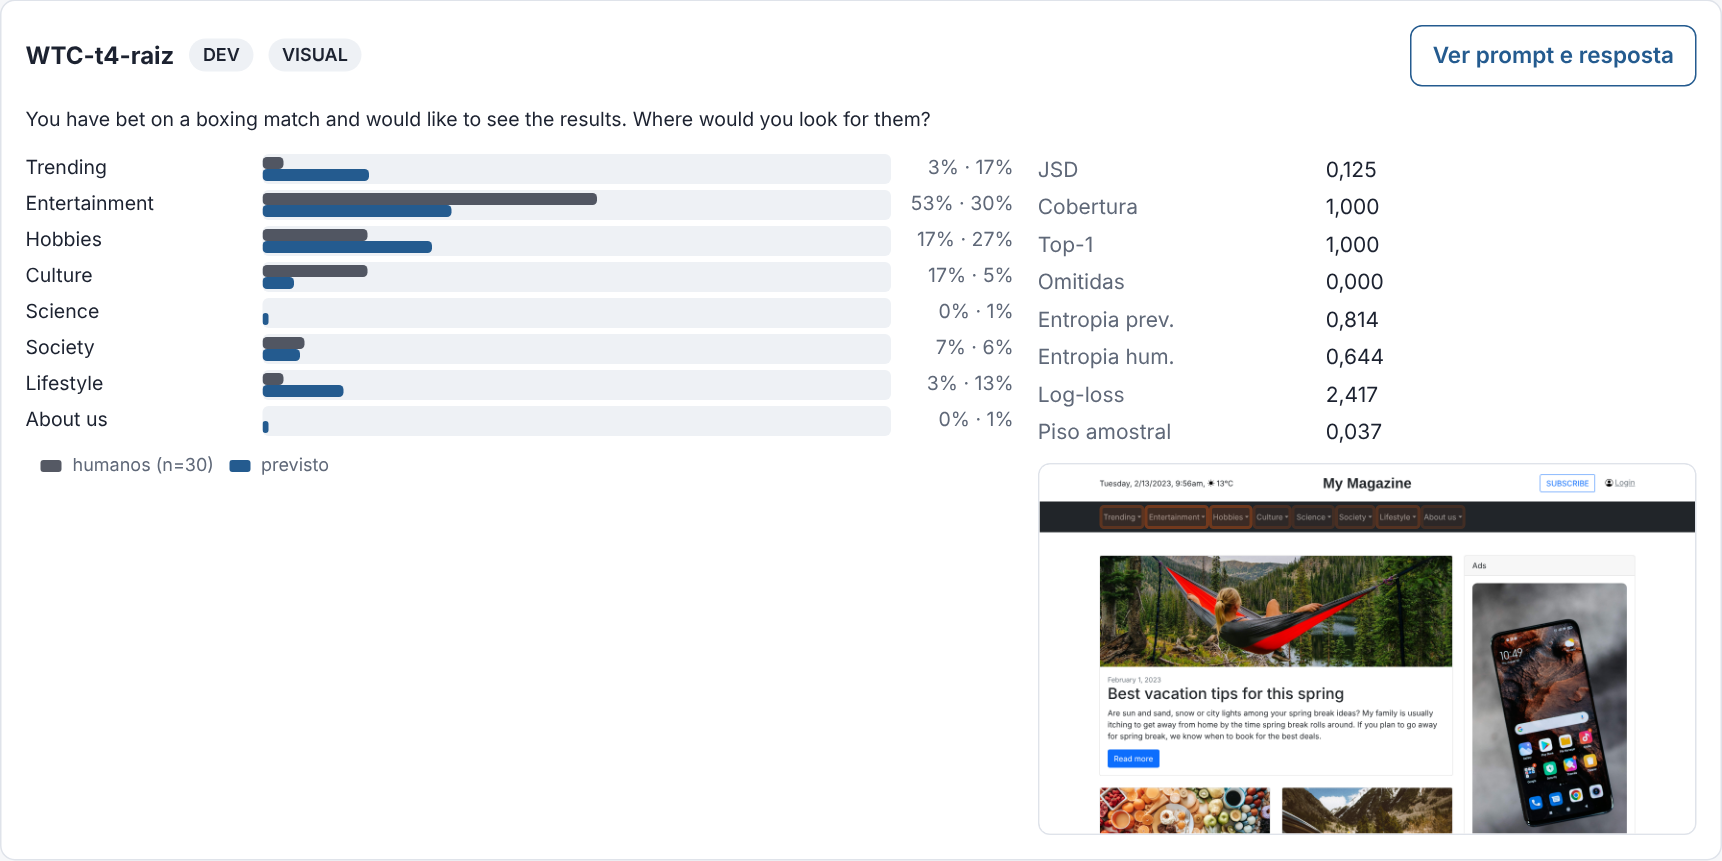
\includegraphics[width=\textwidth]{figuras/painel-previsao-b1cw.png}
\legend{Fonte: captura do protótipo.}
\end{figure}

\section{Etapas do Experimento}
\label{sec:passos}

Esta seção descreve, em ordem, o que é feito em cada etapa e o que cada etapa produz. As etapas 1 a 9 já foram executadas; as demais estão planejadas.

\begin{enumerate}[label=\textbf{Passo \arabic*.},leftmargin=2.1cm,itemsep=3pt]
\item \textbf{Fixar os dados (feito).} Baixar o repositório de \citeonline{kuric2025dataset} na revisão \code{6cc9130}. \emph{Produz:} uma cópia imutável dos dados e dos protótipos.
\item \textbf{Importar e contar (feito).} Para cada uma das 1.800 execuções, tomar o primeiro clique e reduzi-lo à categoria do primeiro nível; descartar as 4 sem clique; agregar por variante e tarefa. \emph{Produz:} 60 estados com contagens humanas, verificados contra uma recontagem independente.
\item \textbf{Renderizar as telas (feito).} Para WTC, WTCI e WM, abrir o protótipo com relógio congelado, extrair as opções e suas coordenadas e salvar a captura. \emph{Produz:} 3 telas idênticas byte a byte em qualquer importação.
\item \textbf{Dividir (feito).} Tarefas pares em DEV e ímpares em TEST. \emph{Produz:} 30 estados de cada lado.
\item \textbf{Montar as entradas (feito).} Para cada estado, gerar o \code{NavInput} (tarefa, opções e tela) e o \textit{hash} da entrada. \emph{Produz:} entradas auditáveis, sem dados humanos.
\item \textbf{Rodar as referências (feito).} UNIFORM e B0, com a temperatura do B0 ajustada só no DEV. \emph{Produz:} previsões, métricas e \textit{hashes} congelados; conferência independente em Python.
\item \textbf{Piloto pequeno com LLMs (feito).} B1 e B1-CW, em Claude e GPT-4.1, em 4 estados do DEV, para verificar prompts, respostas, armazenamento, isolamento das entradas e custo real. \emph{Produz:} o relato da Seção~\ref{sec:piloto}.
\item \textbf{B0 em validação cruzada (feito).} Ajustar a temperatura em cada metade das tarefas e avaliar na outra (Seção~\ref{sec:b0}).
\item \textbf{Análises complementares sem LLM (feito).} Sensibilidade do resultado do B0, poder do teste, referência humana contra o ruído amostral e relação entre erro e entropia humana (Capítulo~\ref{cap:resultados}).
\item \textbf{Decidir os pontos em aberto (planejado).} Versão dos prompts, modelos e demais itens da Seção~\ref{sec:plano}. Ajustes de prompt, se houver, usam só o DEV e geram nova versão.
\item \textbf{Congelar parâmetros e orçamento (planejado).} Registrar versão dos prompts, modelos, esforço, $N$, limiares e semente; estimar o custo a partir dos \textit{tokens} medidos; obter aprovação.
\item \textbf{Rodar as condições B1 uma única vez (planejado).} B1, B1-CW, B1-R, B1-S e B1-CW-S nos dois modelos, em todos os 60 estados (40 entradas distintas), com os parâmetros congelados. Uma rodada de verificação em poucos estados vem antes, para confirmar custo e estabilidade.
\item \textbf{Analisar (planejado).} Diferenças pareadas de H1 a H3 nas 10 tarefas, com os três resumos da Seção~\ref{sec:inferencia} e a correção de Holm; B1 reamostrado para H2; análise por modalidade e variante (H4); análises complementares; custo por ponto de JSD.
\item \textbf{Piloto institucional (planejado).} Capturar a página inicial das tarefas do IFPB, congelar as previsões e só depois coletar as escolhas de iniciantes (Seção~\ref{sec:ifpb}).
\item \textbf{B2, se justificado (planejado).} Comparar um sistema multiagente com o melhor B1, com orçamento equivalente.
\end{enumerate}

\section{Ameaças à Validade e Limitações}
\label{sec:ameacas}

\subsection{Validade interna}

\begin{itemize}
\item \textbf{Vazamento de respostas.} Mitigado pelo isolamento estrutural das entradas, pela captura independente e pela auditoria dos prompts.
\item \textbf{Ajuste no conjunto de avaliação.} A temperatura do B0 é ajustada em validação cruzada, e nenhum estado é avaliado com um $\tau$ ajustado nele. Os prompts das condições com LLM foram escritos antes de qualquer rodada nos dados e só foram testados em 4 estados das tarefas pares; uma eventual revisão gera nova versão e é relatada. Cada condição roda uma única vez.
\item \textbf{Deliberação como confusão.} Pedir Q1 a Q3 também faz o modelo escrever mais. O controle B1-R separa os dois efeitos.
\item \textbf{Contaminação do modelo.} O repositório e o artigo do \textit{benchmark} são públicos desde 2025, e um LLM pode tê-los visto no treino \cite{sainz2023contamination}. Não enviar as contagens no prompt não elimina esse risco. Ele é tratado de duas formas: pela sondagem de memorização descrita na Seção~\ref{sec:complementares} e pelo piloto prospectivo no IFPB, cujos dados ainda não existem e que é o controle definitivo.
\item \textbf{Não determinismo e mudança dos modelos.} As respostas das APIs variam entre chamadas, e o mesmo prompt pode produzir distribuições diferentes com meses de intervalo \cite{bisbee2024synthetic}. Todas as respostas ficam armazenadas, e a análise usa as respostas registradas. A variação entre chamadas é medida no B1-S. Os resultados valem para as versões e datas registradas.
\end{itemize}

\subsection{Validade de construto}

\begin{itemize}
\item O primeiro clique numa categoria do primeiro nível é só o início da navegação. Ele está associado ao sucesso da tarefa \cite{bailey2009firstclick}, mas erros mais profundos e recuperações não são previstos nesta fase.
\item Os participantes do \textit{benchmark} são adultos recrutados \textit{online} e não necessariamente iniciantes no sentido de ingressantes de uma instituição. O \textit{site} é fictício e não é familiar a ninguém, o que aproxima a situação de um primeiro acesso.
\item As condições que analisam cada opção pedem ao modelo um processo exaustivo, que as pessoas não seguem \cite{brumby2008strategies}. O que se avalia é o resultado (a distribuição), e não a semelhança do processo.
\item A JSD resume a distância entre distribuições, mas não diz se o erro está nas opções populares ou nas raras; por isso cobertura e omissões são relatadas junto. A cobertura depende de um limiar, e sua sensibilidade a ele é relatada.
\end{itemize}

\subsection{Validade de conclusão}

Mesmo com 10 tarefas, a amostra de tarefas é pequena. O poder é limitado a efeitos grandes em relação à variação entre tarefas (Seção~\ref{sec:poder}), e o \textit{bootstrap} percentil subestima a incerteza, razão pela qual o intervalo $t$ e o teste exato são exigidos juntos. A correção de Holm é aplicada dentro de cada hipótese, entre os dois modelos, e não entre as hipóteses; H2 e H3 devem ser lidas como secundárias. O resultado já obtido para o B0 mostra a fragilidade de conclusões com dez tarefas: sua significância muda com a forma de escolher a temperatura (Seção~\ref{sec:b0}). O B1-S tem ruído amostral próprio, tratado pela comparação com o B1 reamostrado.

\subsection{Validade externa}

Um \textit{site} de revista em inglês não é um portal institucional em português. Há evidência de que as respostas de LLMs ficam mais próximas de algumas populações do que de outras \cite{santurkar2023whose,durmus2023globalopinions} e de que traduzir a pergunta não basta para aproximá-las da população que fala a língua \cite{durmus2023globalopinions}. A transferência do \textit{benchmark} em inglês para ingressantes brasileiros não pode ser presumida, e é isso que o piloto no IFPB verifica, embora com poucas tarefas. Resultados com dois modelos de 2026 podem não valer para versões futuras.

\section{Considerações Finais do Capítulo}

O método reduz a pergunta de pesquisa a comparações pareadas entre condições que diferem num único fator, sobre a mesma entrada e contra os mesmos dados humanos. As escolhas de desenho mais importantes são três: prever a distribuição, e não o clique mais provável; impedir, pela estrutura do código, que o preditor receba qualquer informação que o iniciante não teria; e analisar por tarefa, com procedimentos adequados a dez agrupamentos e com a limitação de poder declarada de antemão. O capítulo seguinte relata o que já foi executado com esse método.

% =====================================================================
\chapter{Resultados Preliminares e Discussão}
\label{cap:resultados}
% =====================================================================

Este capítulo relata o que já foi executado. Tudo aqui é resultado medido, com dados reais, e pode ser reproduzido pelos comandos do Apêndice~\ref{ap:repro}. O capítulo começa pela validação da implementação. Depois descreve o que os dados humanos mostram, os resultados das duas referências que não usam LLM (UNIFORM e B0), uma análise exploratória da relação entre o erro e a discordância humana e o piloto pequeno com LLMs. A discussão final resume o que esses resultados significam para o experimento completo, que ainda não foi executado.

\section{Validação da Implementação}
\label{sec:validacao}

\begin{real}
Antes de interpretar qualquer métrica, conferimos se o protótipo mede o que diz medir. A Tabela~\ref{tab:validacao} resume as verificações. Todas foram feitas com dados reais; os \textit{scripts} estão no repositório.
\end{real}

\begin{table}[htb]
\centering
\caption{Verificações da implementação.}
\label{tab:validacao}
\scriptsize
\begin{tabularx}{\textwidth}{@{}p{3.0cm}Yp{4.0cm}@{}}
\toprule
\textbf{O que} & \textbf{Como} & \textbf{Resultado} \\
\midrule
Contagens humanas & Recontagem independente em Python, direto do \code{results.csv} bruto & 60/60 estados iguais; textos das tarefas idênticos \\
Tokenizador e \textit{embeddings} do B0 & 12 textos de referência (acentos, pontuação, CJK) contra \code{tokenizers} e \code{onnxruntime} em Python & \textit{Tokens} idênticos; vetores iguais até $10^{-4}$ \\
Temperatura do B0 & Reajuste independente em Python, mesma grade, 30 estados DEV & $\tau=0{,}060912$ nos dois \\
Distribuições do B0 & Recalculadas em Python & Diferença máxima $6\times10^{-7}$ \\
Métricas & Reimplementação independente; JSD via \code{scipy} (base 2, ao quadrado) & Diferença máxima $\approx10^{-15}$ \\
Reprodutibilidade & Duas execuções do zero (banco, armazenamento e modelo novos) e rodadas repetidas & Mesmo \textit{hash} das entradas e mesmos \textit{hashes} congelados \\
Telas & Comparação byte a byte entre importações & WTC, WTCI e WM idênticas \\
Isolamento das entradas & Teste estrutural de \code{NavInput}; auditoria dos 16 prompts do piloto (só tarefa, uma frase sobre a tela e uma linha por opção; todo número vem da tarefa, dos ids ou das coordenadas) & 16/16 limpos \\
\textit{Cache} e custo & Rodada do piloto repetida & 0 chamadas, 0 \textit{tokens}, mesmo \textit{hash} \\
Testes automatizados & JUnit (20 testes) & 19 aprovados; 1 depende do arquivo do modelo de \textit{embeddings} e é ignorado quando ele não está presente \\
\bottomrule
\end{tabularx}
\end{table}

A validação encontrou cinco problemas, todos corrigidos antes dos resultados relatados a seguir:

\begin{enumerate}
\item O anúncio animado do protótipo WTCI tornava a tela diferente a cada importação, o que mudava o \textit{hash} da entrada. Corrigido com relógio simulado e congelado.
\item A concordância top-1 contava empates como acerto, e a previsão uniforme ``acertava'' em 100\% dos estados. Corrigido com o desempate aleatório esperado.
\item No Claude, um esquema com o campo \code{thought} disparava recusas por ``extração de raciocínio''. O campo foi renomeado para \code{reason}, e recusas passaram a ser contadas sem interromper a rodada.
\item A ordem das chaves do esquema JSON variava entre execuções da JVM, mudando a chave de \textit{cache} e o \textit{hash} do prompt. Corrigido com mapas ordenados.
\item Rodadas servidas pelo \textit{cache} somavam \textit{tokens} como se tivessem sido gastos. Corrigido para contar só o que foi efetivamente chamado.
\end{enumerate}

\section{O que os Dados Humanos Mostram}
\label{sec:humanos}

\subsection{As escolhas são dispersas}

\begin{real}
Nos 60 estados, a opção mais escolhida reúne em média 58\% das pessoas, e em 28\% dos estados (17 de 60) nenhuma opção chega a 50\%. Há em média 2,6 opções escolhidas por pelo menos 10\% das pessoas (mínimo 1, máximo 4). A entropia normalizada humana média é 0,515, com intervalo de 95\% de [0,441; 0,585] por \textit{bootstrap} de tarefas.
\end{real}

Esses números confirmam a premissa do trabalho: no primeiro clique, a pergunta relevante é como as pessoas se repartem entre duas ou três opções plausíveis, e a resposta ``qual é a opção certa'' descreve só pouco mais da metade delas.

\subsection{Acertar a opção mais escolhida não basta}

\begin{real}
Para medir quanto vale acertar o primeiro lugar, construímos uma previsão artificial que usa os próprios dados humanos: toda a probabilidade na opção mais escolhida de cada estado. Essa previsão tem concordância top-1 igual a 1 em todos os estados, por construção. Ainda assim, sua JSD média é 0,259 [0,198; 0,324], e sua cobertura é de apenas 0,582, porque ela ignora todas as pessoas que foram para outra opção.
\end{real}

O valor de 0,259 é só um pouco menor que o do B0 (0,288, Seção~\ref{sec:b0}), que acerta a opção mais escolhida em menos da metade dos estados. Um preditor que colapsa na resposta ``certa'' fica, portanto, longe da distribuição humana mesmo quando nunca erra o primeiro lugar. É o comportamento de ``super-usuário'' levado ao limite, e mostra por que a métrica principal precisa olhar a distribuição inteira.

\subsection{Até onde um preditor pode chegar}

\begin{real}
O piso amostral da JSD, com 30 pessoas por estado, é 0,028 [0,024; 0,031] nas 10 tarefas (0,027 no TEST). A referência humana entre variantes, isto é, a distribuição da mesma tarefa nas outras cinco variantes, tem JSD de 0,044 nas 10 tarefas (0,043 [0,040; 0,047] no TEST; 0,039 nas variantes textuais e 0,048 nas visuais).

A referência (0,044) é maior que o piso (0,028). Parte dessa diferença é esperada mesmo sem nenhum efeito da apresentação, porque a referência compara duas amostras finitas, e as duas têm ruído. Para medir quanto, embaralhamos as escolhas de cada tarefa entre as seis variantes, mantendo o tamanho de cada grupo, e recalculamos a referência 2.000 vezes. O valor esperado sem efeito da apresentação é 0,045, e o valor observado (0,044) fica dentro do que o acaso produz ($p=0{,}65$).
\end{real}

Duas leituras decorrem desse resultado. A primeira é que, neste \textit{benchmark} e no primeiro clique do primeiro nível, a variação das escolhas entre as seis apresentações não se distingue do ruído de amostras de 30 pessoas. A distribuição depende da tarefa e da arquitetura de informação; um efeito da apresentação, se existe, é pequeno demais para aparecer com esse tamanho de amostra. Isso vale para o primeiro clique e não diz nada sobre outras medidas do estudo original, como o caminho percorrido ou o sucesso da tarefa. A segunda leitura é que a meta realista de um bom preditor é a faixa entre o piso e a referência, de cerca de 0,03 a 0,045 de JSD. Abaixo disso, não há como distinguir um preditor melhor de um preditor igualmente bom.

O resultado também afeta a QP4. Como as distribuições humanas quase não mudam entre texto e protótipo visual, uma diferença de desempenho de um preditor entre as modalidades dirá mais sobre o preditor (por exemplo, sobre como ele usa a imagem) do que sobre as pessoas.

\section{Referências sem LLM: UNIFORM e B0}
\label{sec:b0}

\subsection{Rodada congelada}

\begin{real}
A Tabela~\ref{tab:b0} traz os resultados da rodada congelada de B0 e UNIFORM, em que a temperatura do B0 foi ajustada no DEV: $\tau=0{,}0609$, com JSD média de 0,281 no DEV. \textit{Hashes} congelados: UNIFORM \code{7763c445\ldots}, B0 \code{55de6c0f\ldots}.
\end{real}

\begin{table}[htb]
\centering
\caption{UNIFORM e B0 na rodada congelada (média e IC 95\% por \textit{bootstrap} de tarefas). A seta indica se o melhor valor é o menor ($\downarrow$) ou o maior ($\uparrow$).}
\label{tab:b0}
\scriptsize\setlength{\tabcolsep}{4pt}
\begin{tabular}{@{}llccccc@{}}
\toprule
\textbf{Grupo} & \textbf{Método} & \textbf{JSD $\downarrow$} & \textbf{Cobertura $\uparrow$} & \textbf{Top-1 $\uparrow$} & \textbf{Omitidas $\downarrow$} & \textbf{Entropia prev.} \\
\midrule
TEST, todos & UNIFORM & 0,378 [0,352; 0,402] & 1,000 & 0,133 & 0,00 & 1,000 \\
TEST, todos & B0 & 0,289 [0,217; 0,387] & 0,948 [0,913; 0,975] & 0,433 [0,03; 0,83] & 0,20 & 0,858 \\
TEST, texto & UNIFORM & 0,401 [0,392; 0,413] & 1,000 & 0,133 & 0,00 & 1,000 \\
TEST, texto & B0 & 0,308 [0,215; 0,425] & 0,958 & 0,467 & 0,13 & 0,858 \\
TEST, visual & UNIFORM & 0,354 [0,307; 0,402] & 1,000 & 0,133 & 0,00 & 1,000 \\
TEST, visual & B0 & 0,271 [0,205; 0,357] & 0,938 & 0,400 & 0,27 & 0,858 \\
DEV, todos & B0 & 0,281 [0,202; 0,344] & 0,927 & 0,400 & 0,27 & 0,814 \\
\midrule
\multicolumn{7}{@{}l}{\textit{Log-loss} no TEST: UNIFORM 3,000 bits; B0 2,615 [2,169; 3,205] bits.} \\
\bottomrule
\end{tabular}
\end{table}

\begin{real}
A diferença pareada B0 $-$ UNIFORM na JSD é $-0{,}088$ [$-0{,}172$; $+0{,}029$] no TEST e $-0{,}091$ [$-0{,}149$; $-0{,}020$] no DEV. No TEST, o intervalo cruza zero: com cinco tarefas, não se pode afirmar que o B0 é melhor que o acaso fora do conjunto em que foi ajustado. No DEV a diferença é significativa, mas a temperatura foi ajustada ali.
\end{real}

\subsection{B0 em validação cruzada, nas 10 tarefas}

\begin{real}
Ajustando $\tau$ nas tarefas pares ($\tau=0{,}0609$, o mesmo da rodada) e aplicando às ímpares, e ajustando nas ímpares ($\tau=0{,}0451$) e aplicando às pares, obtêm-se os valores da Tabela~\ref{tab:b0cv}. A diferença pareada é $-0{,}087$, com intervalo por \textit{bootstrap} de [$-0{,}145$; $-0{,}017$] e intervalo $t$ de [$-0{,}165$; $-0{,}008$]. O B0 fica abaixo do UNIFORM em 8 das 10 tarefas, com $p=0{,}041$ no teste exato de troca de sinal. Só com as 5 tarefas ímpares, o mesmo teste dá $p=0{,}25$, e nunca poderia ficar abaixo de 0,0625. O efeito do B0 já era o mesmo ($-0{,}088$ só nas ímpares); o que mudou foi a capacidade de detectá-lo. Cálculo em \code{analysis/nav\_b0\_crossfit.py}, sem chamadas a LLMs.
\end{real}

\begin{table}[htb]
\centering
\caption{B0 com temperatura em validação cruzada e UNIFORM, nas 10 tarefas (média e IC 95\% por \textit{bootstrap} de tarefas).}
\label{tab:b0cv}
\footnotesize
\begin{tabular}{@{}lccc@{}}
\toprule
\textbf{Grupo} & \textbf{JSD do UNIFORM} & \textbf{JSD do B0} & \textbf{B0 $-$ UNIFORM} \\
\midrule
Todos os 60 estados & 0,375 [0,330; 0,420] & 0,288 [0,239; 0,345] & $-0{,}087$ [$-0{,}145$; $-0{,}017$] \\
Variantes textuais & 0,401 [0,350; 0,457] & 0,308 [0,248; 0,376] & $-0{,}093$ [$-0{,}149$; $-0{,}026$] \\
Variantes visuais & 0,349 [0,306; 0,391] & 0,269 [0,224; 0,320] & $-0{,}080$ [$-0{,}140$; $-0{,}008$] \\
\midrule
\multicolumn{4}{@{}p{0.92\textwidth}@{}}{Outras métricas do B0 nos 60 estados: cobertura 0,882 [0,785; 0,954]; opções omitidas 0,48 [0,17; 0,90]; top-1 0,417 [0,117; 0,717]; entropia prevista 0,792 [0,695; 0,872].} \\
\bottomrule
\end{tabular}
\end{table}

A Figura~\ref{fig:variantes} mostra a JSD por variante. Como o B0 só usa texto, ele prevê a mesma distribuição para as seis variantes de uma tarefa; as diferenças entre variantes vêm só dos humanos.

\begin{figure}[htb]
\centering
\caption{JSD por variante, nos 10 estados de cada uma, com a temperatura do B0 em validação cruzada. Linhas tracejadas: piso amostral (0,028) e referência humana entre variantes (0,044).}
\label{fig:variantes}
\begin{tikzpicture}
\begin{axis}[
  ybar, bar width=10pt, width=0.92\textwidth, height=5.8cm, enlarge x limits=0.12,
  ymin=0, ymax=0.48, ylabel={JSD média (10 tarefas)},
  symbolic x coords={TP,TC,TO,WTC,WTCI,WM}, xtick=data,
  legend style={at={(0.5,1.03)},anchor=south,legend columns=-1,font=\footnotesize},
  ticklabel style={font=\footnotesize}, label style={font=\footnotesize},
  nodes near coords, nodes near coords style={font=\tiny, /pgf/number format/fixed, /pgf/number format/precision=2},
  extra y ticks={0.028,0.044}, extra y tick labels={,},
  extra y tick style={grid=major, grid style={dashed, gray}}
]
\addplot[fill=gray!40] coordinates {(TP,0.374) (TC,0.410) (TO,0.419) (WTC,0.345) (WTCI,0.365) (WM,0.336)};
\addplot[fill=blue!45] coordinates {(TP,0.290) (TC,0.304) (TO,0.329) (WTC,0.260) (WTCI,0.293) (WM,0.254)};
\legend{UNIFORM, B0}
\end{axis}
\end{tikzpicture}
\legend{Fonte: elaborada pelo autor.}
\end{figure}

\subsection{O resultado depende de como a temperatura é escolhida}
\label{sec:sensibilidade}

O valor de $p=0{,}041$ fica perto do limiar, e por isso verificamos quanto ele depende do único parâmetro ajustado, a temperatura.

\begin{real}
A Tabela~\ref{tab:sensib} repete a comparação com outras formas de escolher $\tau$. A direção do resultado é estável: em todas, o B0 fica abaixo do acaso em 8 ou 9 das 10 tarefas, com diferença média entre $-0{,}06$ e $-0{,}09$. A significância não é estável: o valor de $p$ vai de 0,006 a 0,28.
\end{real}

\begin{table}[htb]
\centering
\caption{Diferença B0 $-$ UNIFORM nas 10 tarefas, conforme a forma de escolher a temperatura do B0. O valor de $p$ é o do teste exato de troca de sinal.}
\label{tab:sensib}
\footnotesize
\begin{tabular}{@{}lccc@{}}
\toprule
\textbf{Como $\tau$ é escolhida} & \textbf{Diferença média} & \textbf{Tarefas com B0 melhor} & \textbf{$p$} \\
\midrule
Validação cruzada em duas partes (protocolo) & $-0{,}087$ & 8 de 10 & 0,041 \\
Ajuste deixando a própria tarefa de fora & $-0{,}073$ & 8 de 10 & 0,127 \\
\midrule
Fixa, $\tau=0{,}030$ & $-0{,}070$ & 8 de 10 & 0,283 \\
Fixa, $\tau=0{,}045$ & $-0{,}088$ & 8 de 10 & 0,080 \\
Fixa, $\tau=0{,}061$ & $-0{,}090$ & 8 de 10 & 0,031 \\
Fixa, $\tau=0{,}080$ & $-0{,}084$ & 8 de 10 & 0,014 \\
Fixa, $\tau=0{,}100$ & $-0{,}077$ & 8 de 10 & 0,012 \\
Fixa, $\tau=0{,}150$ & $-0{,}060$ & 9 de 10 & 0,006 \\
\bottomrule
\end{tabular}
\end{table}

A explicação está nas duas tarefas em que o B0 erra a direção (7 e 8). Com temperatura baixa, o B0 concentra a probabilidade na opção que prefere; quando essa opção está errada, a perda nessas tarefas é grande e aumenta a variação entre tarefas. Com temperatura alta, o B0 se aproxima do acaso: ganha menos onde acerta, mas perde muito menos onde erra, e a vantagem fica mais regular. A temperatura que minimiza a JSD média não é, portanto, a que dá a vantagem mais consistente.

A conclusão sustentada pelos dados é mais modesta do que ``o B0 é significativamente melhor que o acaso''. O B0 é melhor que o acaso na maioria das tarefas, por uma margem de 0,06 a 0,09 de JSD, e a análise definida no protocolo dá $p=0{,}041$. Esse valor não resiste a mudanças razoáveis na escolha da temperatura, e o resultado deve ser lido como evidência moderada. As linhas de temperatura fixa da tabela são análises feitas depois de ver os dados e servem só para mostrar a sensibilidade.

\subsection{Onde o B0 erra}

\begin{real}
A Tabela~\ref{tab:b0erros} compara, tarefa a tarefa, a previsão do B0 com as escolhas humanas agregadas nas seis variantes (cerca de 180 pessoas por tarefa). O B0 acerta a opção mais escolhida em 4 das 10 tarefas. Ele é mais disperso que os humanos em 9 das 10: a entropia normalizada média do B0 é 0,79, contra 0,55 dos humanos agregados.
\end{real}

\begin{table}[htb]
\centering
\caption{B0 (validação cruzada) contra as escolhas humanas agregadas nas seis variantes, por tarefa. ``B0 na opção humana'' é a probabilidade que o B0 deu à opção mais escolhida pelas pessoas.}
\label{tab:b0erros}
\scriptsize\setlength{\tabcolsep}{4pt}
\begin{tabularx}{\textwidth}{@{}Yllccc@{}}
\toprule
\textbf{Tarefa} & \textbf{Mais escolhida} & \textbf{Mais provável} & \textbf{B0 na opção} & \textbf{Entropia} & \textbf{B0 $-$} \\
 & \textbf{(humanos)} & \textbf{(B0)} & \textbf{humana} & \textbf{hum. / B0} & \textbf{UNIFORM} \\
\midrule
2, filme de comédia & Entertainment (0,85) & Hobbies (0,51) & 0,24 & 0,30 / 0,68 & $-0{,}149$ \\
3, cinemas próximos & Entertainment (0,75) & Entertainment (0,35) & 0,35 & 0,46 / 0,85 & $-0{,}214$ \\
4, resultado de luta de boxe & Entertainment (0,63) & Science (0,26) & 0,21 & 0,56 / 0,90 & $-0{,}043$ \\
5, receita mesoamericana & Lifestyle (0,36) & Culture (0,21) & 0,20 & 0,63 / 0,92 & $-0{,}145$ \\
6, renovar o guarda-roupa & Lifestyle (0,52) & Lifestyle (0,69) & 0,69 & 0,67 / 0,43 & $-0{,}133$ \\
7, vida na Idade Média & Culture (0,60) & Lifestyle (0,48) & 0,09 & 0,59 / 0,70 & $+0{,}137$ \\
8, comprar um \textit{laptop} & Lifestyle (0,28) & Trending (0,37) & 0,24 & 0,77 / 0,83 & $+0{,}065$ \\
9, espécies de aves & Science (0,56) & Lifestyle (0,29) & 0,21 & 0,57 / 0,89 & $-0{,}097$ \\
10, doenças e sintomas & Lifestyle (0,54) & Lifestyle (0,42) & 0,42 & 0,48 / 0,79 & $-0{,}166$ \\
11, cuidar de um bebê & Lifestyle (0,64) & Lifestyle (0,25) & 0,25 & 0,51 / 0,93 & $-0{,}122$ \\
\bottomrule
\end{tabularx}
\end{table}

O B0 segue a semelhança literal entre palavras, e não o modelo mental do leitor. Na tarefa 7 (vida na Idade Média), o B0 prefere Lifestyle, provavelmente porque o enunciado fala em ``life'', enquanto 60\% das pessoas escolhem Culture; é a tarefa em que o B0 mais perde para o acaso. Na tarefa 2 (filme de comédia para uma noite com amigos), 85\% das pessoas escolhem Entertainment, e o B0 põe Hobbies em primeiro. Esta análise de erros foi feita depois de as previsões do B0 estarem congeladas e não alimenta nenhum ajuste.

O padrão de erro do B0 é o oposto do relatado para LLMs. O B0 espalha a probabilidade demais e erra a ordem das opções; os LLMs, segundo a literatura, concentram demais \cite{kuric2026wwgc}. Os casos em que o B0 falha são os que um preditor com conhecimento de mundo deveria resolver, e é isso que H3 testa.

\section{Análise Exploratória: Erro e Discordância Humana}
\label{sec:entropia}

Uma pergunta natural é se os preditores erram mais nos estados em que as pessoas mais discordam entre si \cite{lee2023dissenting}. Esta seção faz essa análise para o B0 e o UNIFORM. Ela é exploratória, foi feita depois de ver os dados e não testa nenhuma hipótese. Serve para preparar a leitura da mesma análise nas condições com LLM.

\begin{real}
A Figura~\ref{fig:entropia} mostra, para cada um dos 60 estados, a entropia normalizada humana e a JSD das duas referências. A JSD do UNIFORM cai de forma quase mecânica quando a entropia humana sobe (correlação de Spearman de $-0{,}97$): quanto mais as pessoas se espalham, mais a distribuição humana se parece com o acaso. A JSD do B0 também cai, mas menos ($-0{,}42$, com intervalo de 95\% de [$-0{,}78$; $-0{,}14$] por \textit{bootstrap} de tarefas). Como consequência, a vantagem do B0 sobre o acaso encolhe à medida que a entropia sobe (correlação de $+0{,}48$ [$+0{,}19$; $+0{,}69$] entre a entropia e a diferença B0 $-$ UNIFORM). A Tabela~\ref{tab:tercis} resume o padrão em três faixas.
\end{real}

\begin{figure}[htb]
\centering
\caption{Entropia normalizada humana e JSD em cada um dos 60 estados, para o UNIFORM e para o B0 (validação cruzada). Cada ponto é um estado.}
\label{fig:entropia}
\begin{tikzpicture}
\begin{axis}[
  width=0.88\textwidth, height=6.4cm, xmin=0, xmax=0.85, ymin=0, ymax=0.7,
  xlabel={entropia normalizada das escolhas humanas no estado}, ylabel={JSD},
  legend style={at={(0.98,0.97)},anchor=north east,font=\footnotesize},
  ticklabel style={font=\footnotesize}, label style={font=\footnotesize},
  /pgf/number format/use comma
]
\addplot[only marks, mark=o, mark size=1.6pt, gray!70!black] coordinates {(0.225,0.559) (0.448,0.394) (0.539,0.349) (0.558,0.377) (0.657,0.274) (0.594,0.318) (0.699,0.263) (0.522,0.362) (0.487,0.418) (0.462,0.426) (0.070,0.661) (0.457,0.379) (0.417,0.423) (0.523,0.421) (0.619,0.305) (0.392,0.462) (0.735,0.222) (0.481,0.409) (0.392,0.462) (0.539,0.355) (0.187,0.578) (0.391,0.411) (0.482,0.412) (0.577,0.369) (0.610,0.314) (0.475,0.403) (0.678,0.282) (0.370,0.503) (0.390,0.496) (0.472,0.422) (0.448,0.394) (0.338,0.476) (0.644,0.275) (0.729,0.228) (0.585,0.307) (0.521,0.365) (0.793,0.175) (0.556,0.350) (0.503,0.405) (0.338,0.476) (0.225,0.559) (0.525,0.349) (0.351,0.478) (0.588,0.356) (0.708,0.235) (0.625,0.311) (0.580,0.368) (0.655,0.271) (0.511,0.397) (0.591,0.324) (0.423,0.407) (0.374,0.458) (0.665,0.251) (0.577,0.369) (0.623,0.285) (0.683,0.223) (0.803,0.169) (0.634,0.306) (0.450,0.443) (0.394,0.451)};
\addplot[only marks, mark=*, mark size=1.6pt, blue!70!black] coordinates {(0.225,0.419) (0.448,0.175) (0.539,0.330) (0.558,0.243) (0.657,0.236) (0.594,0.412) (0.699,0.231) (0.522,0.238) (0.487,0.321) (0.462,0.292) (0.070,0.474) (0.457,0.167) (0.417,0.343) (0.523,0.249) (0.619,0.132) (0.392,0.596) (0.735,0.242) (0.481,0.342) (0.392,0.227) (0.539,0.265) (0.187,0.425) (0.391,0.178) (0.482,0.364) (0.577,0.230) (0.610,0.083) (0.475,0.561) (0.678,0.432) (0.370,0.367) (0.390,0.348) (0.472,0.303) (0.448,0.223) (0.338,0.258) (0.644,0.299) (0.729,0.109) (0.585,0.140) (0.521,0.512) (0.793,0.219) (0.556,0.247) (0.503,0.244) (0.338,0.348) (0.225,0.461) (0.525,0.139) (0.351,0.381) (0.588,0.189) (0.708,0.178) (0.625,0.525) (0.580,0.478) (0.655,0.183) (0.511,0.212) (0.591,0.182) (0.423,0.262) (0.374,0.269) (0.665,0.214) (0.577,0.234) (0.623,0.154) (0.683,0.297) (0.803,0.262) (0.634,0.244) (0.450,0.272) (0.394,0.330)};
\legend{UNIFORM, B0}
\end{axis}
\end{tikzpicture}
\legend{Fonte: elaborada pelo autor.}
\end{figure}

\begin{table}[htb]
\centering
\caption{JSD do UNIFORM e do B0 por faixa de entropia humana (20 estados em cada faixa).}
\label{tab:tercis}
\footnotesize
\begin{tabular}{@{}lccccc@{}}
\toprule
\textbf{Entropia humana} & \textbf{UNIFORM} & \textbf{B0} & \textbf{B0 $-$ UNIFORM} & \textbf{B0 pior que o acaso} & \textbf{Top-1 do B0} \\
\midrule
Baixa (0,07 a 0,46) & 0,473 & 0,326 & $-0{,}147$ & 1 de 20 & 0,50 \\
Média (0,46 a 0,58) & 0,382 & 0,297 & $-0{,}084$ & 3 de 20 & 0,45 \\
Alta (0,59 a 0,80) & 0,269 & 0,241 & $-0{,}028$ & 8 de 20 & 0,30 \\
\bottomrule
\end{tabular}
\end{table}

A tabela mostra por que essa análise precisa de cuidado. Olhando só a JSD absoluta, o B0 parece \emph{melhor} quando as pessoas discordam (0,241 contra 0,326). Olhando a diferença para o acaso, parece \emph{pior} ($-0{,}028$ contra $-0{,}147$). As duas leituras são verdadeiras e medem coisas diferentes. Quando as pessoas se espalham, qualquer previsão espalhada fica mais perto delas, inclusive o acaso, e por isso o acaso se torna uma referência difícil de superar. O B0 fica pior que o acaso em 12 dos 60 estados, todos das tarefas 4, 7 e 8, e 8 deles estão na faixa de entropia alta. Quando as pessoas concordam, o B0 ganha do acaso por ser menos uniforme, mas ainda erra a opção mais escolhida em metade dos estados.

Para o experimento completo, a consequência é metodológica. A relação entre o erro de uma condição com LLM e a entropia humana não pode ser lida sozinha: ela será sempre apresentada ao lado da curva do UNIFORM e do piso amostral, como na Figura~\ref{fig:entropia}.

\section{Piloto Pequeno com LLMs}
\label{sec:piloto}

\begin{real}
\textbf{Desenho.} Quatro estados do DEV, escolhidos para cobrir os casos: TP-t2 (texto, humanos concentrados), TP-t8 (texto, humanos dispersos), WTC-t4 (visual, \textit{desktop}) e WM-t8 (visual, celular, humanos dispersos). B1 e B1-CW, uma chamada por estado, em Claude Opus~5.5 e GPT-4.1, esforço \code{medium}, prompts \code{nav-1.1}. Nenhum estado do TEST foi enviado a LLMs. A Tabela~\ref{tab:piloto} traz as médias e a Tabela~\ref{tab:pilotoestados}, os estados.
\end{real}

\begin{table}[htb]
\centering
\caption{Piloto: médias nos 4 estados DEV. Custo estimado por preço de tabela (Claude US\$~4/20 e GPT-4.1 US\$~2/8 por milhão de \textit{tokens} de entrada/saída; o preço do GPT-4.1 ainda precisa ser conferido).}
\label{tab:piloto}
\scriptsize
\begin{tabular}{@{}llcccccc@{}}
\toprule
\textbf{Método} & \textbf{Modelo} & \textbf{JSD $\downarrow$} & \textbf{Cobertura $\uparrow$} & \textbf{Top-1 $\uparrow$} & \textbf{Entropia prev.} & \textbf{\textit{Tokens} (ent./saída)} & \textbf{Custo} \\
\midrule
B0 & -- & 0,285 & 0,958 & 0,00 & 0,88 & -- & 0 \\
B1 & Claude Opus 5.5 & 0,131 & 0,942 & 0,25 & 0,69 & 4.612 / 937 & US\$ 0,037 \\
B1-CW & Claude Opus 5.5 & 0,119 & 0,933 & 0,50 & 0,70 & 6.572 / 2.018 & US\$ 0,067 \\
B1 & GPT-4.1 & 0,195 & 0,875 & 0,38 & 0,72 & 2.839 / 964 & US\$ 0,013 \\
B1-CW & GPT-4.1 & 0,248 & 0,725 & 0,50 & 0,54 & 3.695 / 1.693 & US\$ 0,021 \\
\bottomrule
\end{tabular}
\end{table}

\begin{table}[htb]
\centering
\caption{Piloto, por estado: JSD e destaque de cada estado. Humanos: as opções com pelo menos 4 escolhas.}
\label{tab:pilotoestados}
\scriptsize
\begin{tabularx}{\textwidth}{@{}p{1.2cm}p{3.0cm}cccccY@{}}
\toprule
\textbf{Estado} & \textbf{Humanos ($n=30$)} & \textbf{B0} & \textbf{B1 Cl.} & \textbf{B1-CW Cl.} & \textbf{B1 GPT} & \textbf{B1-CW GPT} & \textbf{Destaque} \\
\midrule
TP-t2 & Entertainment 26 & 0,416 & 0,082 & 0,075 & 0,187 & 0,173 & B0 erra a opção mais escolhida (Hobbies); LLMs acertam. \\
TP-t8 & Lifestyle 12, Hobbies 7, Entertainment 5, Science 4 & 0,218 & 0,149 & 0,160 & 0,181 & 0,198 & Claude põe Science em 1º (0,40): viés de ``especialista''. \\
WTC-t4 & Entertainment 16, Hobbies 5, Culture 5 & 0,285 & 0,144 & 0,125 & 0,243 & 0,359 & GPT põe Trending em 1º; B1-CW concentra mais. \\
WM-t8 & Hobbies 8, Entertainment 7, Science 7, Lifestyle 5 & 0,219 & 0,148 & 0,118 & 0,170 & 0,261 & Distribuição humana muito dispersa. \\
\bottomrule
\end{tabularx}
\end{table}

\begin{real}
\textbf{O que o piloto indica.} São quatro estados, e nada aqui é teste de hipótese.

O B1, nos dois modelos, e o B1-CW do Claude ficaram abaixo do B0 em JSD nos quatro estados. O B1-CW do GPT-4.1 ficou acima do B0 em dois (WTC-t4 e WM-t8).

O efeito de Q1 a Q3 mudou de direção conforme o modelo. No Claude, o B1-CW reduziu a JSD em 3 de 4 estados (de 0,131 para 0,119). No GPT-4.1, aumentou em 3 de 4 (de 0,195 para 0,248), reduzindo a entropia (de 0,72 para 0,54) e a cobertura (de 0,875 para 0,725). As perguntas deixaram o GPT mais concentrado. É o tipo de interação entre modelo e condição que H1 precisa testar com todos os estados.

Armazenamento e auditoria funcionaram: 16 previsões, 0 respostas inválidas, 0 recusas, prompts limpos.

O custo do piloto foi de cerca de US\$~0,14 estimado (16 chamadas). Os testes de funcionamento anteriores (5 estados, incluindo amostragem) custaram cerca de US\$~0,60 estimados. O custo real é o do painel de faturamento de cada fornecedor.
\end{real}

\begin{real}
\textbf{Amostragem (teste de funcionamento).} Em testes de funcionamento do B1-S com poucas amostras (5 estados DEV; $N=3$ no Claude e $N=5$ no GPT-4.1), os dois LLMs deram quase sempre a mesma escolha para o mesmo estado: entropia prevista de 0,00 (Claude) e 0,05 (GPT-4.1), com JSD de 0,50 e 0,47. É a subdispersão relatada por \citeonline{kuric2026wwgc} e é compatível com o que \citeonline{park2024diminished} chamam de efeito da resposta correta. Com $N$ tão pequeno, isso é só um indício; a medida está prevista no experimento completo.
\end{real}

\begin{real}
\textbf{Duas verificações feitas sobre as respostas do piloto, sem novas chamadas.}

\textit{Quanto custa amostrar.} Sorteando 30 escolhas da própria distribuição declarada pelo modelo, a JSD sobe em média 0,03 nas quatro rodadas (entre $+0{,}032$ e $+0{,}035$), só pelo ruído de ter 30 amostras. É a mesma ordem do piso amostral. Isso confirma a necessidade do B1 reamostrado na comparação de H2: sem ele, o B1-S pareceria pior que o B1 por uma margem de 0,03 mesmo que se comportasse de forma idêntica.

\textit{Probabilidades no limiar.} Os modelos declararam probabilidades arredondadas, e em três das quatro rodadas duas das 32 probabilidades foram exatamente 0,05, o valor do limiar de cobertura. A cobertura dessas rodadas depende, portanto, de o limiar ser inclusivo. Por isso a sensibilidade da cobertura ao limiar entra nas análises complementares (Seção~\ref{sec:complementares}).
\end{real}

\begin{figure}[htb]
\centering
\caption{Painel: comparação das rodadas no \textit{benchmark} (métricas, custo e \textit{hash} congelado de cada rodada).}
\label{fig:comparacao}
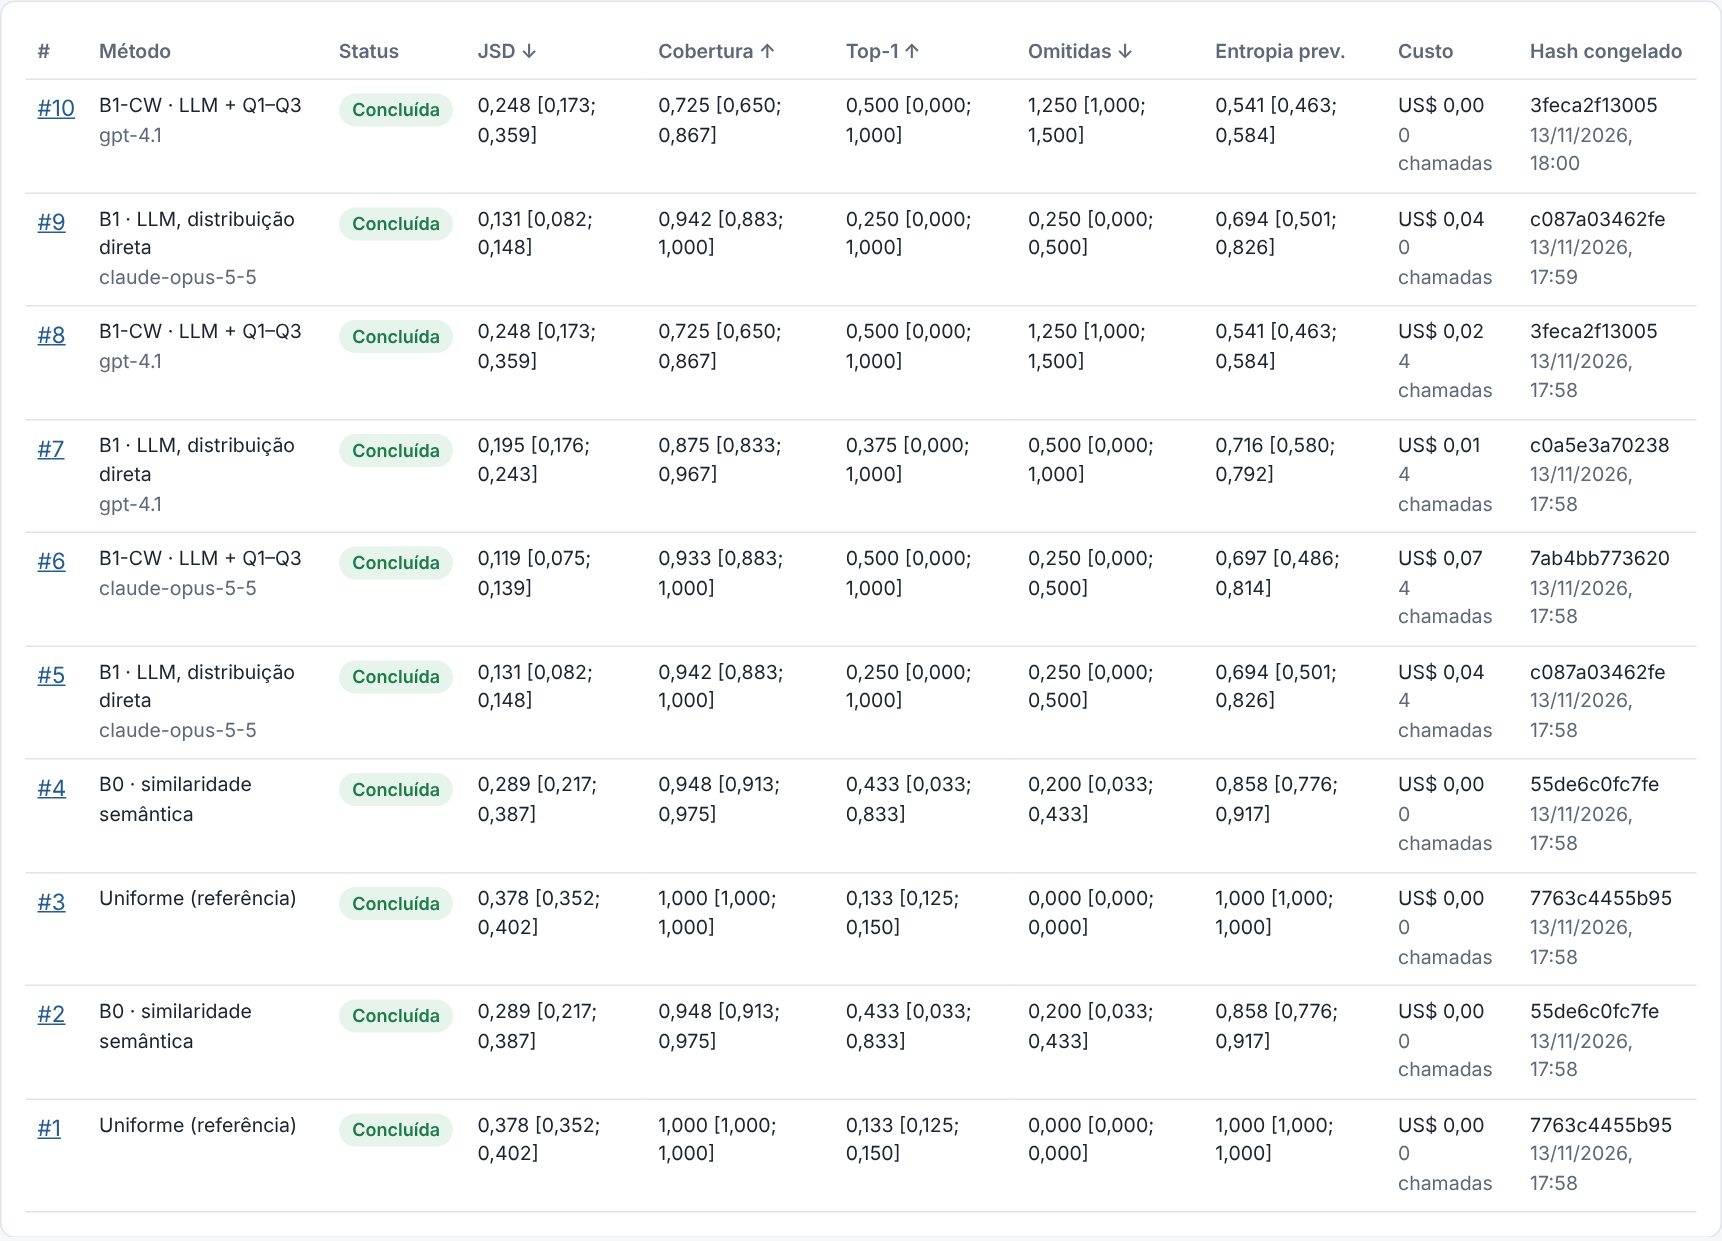
\includegraphics[width=\textwidth]{figuras/painel-comparacao.png}
\legend{Fonte: captura do protótipo.}
\end{figure}

\section{Discussão}
\label{sec:discussao}

Os resultados deste capítulo não respondem ainda às questões de pesquisa, que dependem do experimento completo. Eles estabelecem o terreno em que as respostas serão lidas, e cinco pontos merecem destaque.

\textbf{A meta está definida.} Um preditor ideal ficaria entre 0,03 e 0,045 de JSD, a faixa em que estão o piso amostral e a distância entre duas amostras humanas da mesma tarefa. O acaso está em 0,375 e a \textit{baseline} semântica em 0,288. Há, portanto, um intervalo grande entre o que um método simples alcança e o que os dados permitem alcançar, e é nesse intervalo que as condições com LLM serão situadas (QP1).

\textbf{Acertar o primeiro lugar não é o objetivo.} Uma previsão que põe tudo na opção mais escolhida de cada estado, usando os dados humanos, fica em 0,259. Um preditor que concentre toda a probabilidade numa única opção, como um ``super-usuário'', não passa desse valor, por melhor que seja a sua escolha. Qualquer ganho além disso exige prever a repartição entre as opções, o que dá sentido prático às QP2 e QP3.

\textbf{A \textit{baseline} erra por excesso de dispersão.} O B0 é melhor que o acaso em 8 das 10 tarefas, mas espalha a probabilidade demais e acerta a opção mais escolhida em só 4 tarefas. O erro esperado dos LLMs é o contrário. As métricas de dispersão e de omissão vão mostrar se os LLMs trocam um erro pelo outro ou se chegam mais perto da repartição humana.

\textbf{Dez tarefas sustentam poucas conclusões.} O resultado do B0 contra o acaso tem $p=0{,}041$ pela análise do protocolo e deixa de ser significativo com outra forma de escolher a temperatura. O poder do teste só alcança efeitos da ordem da variação entre tarefas. No piloto, o efeito das perguntas do percurso cognitivo no Claude foi de $-0{,}011$, muito abaixo do que o desenho detecta com segurança, e no GPT-4.1 foi de $+0{,}053$, na direção contrária. A leitura de H1 terá de separar três situações: efeito detectado, efeito não detectado com intervalo estreito e efeito não detectado com intervalo largo. Só a segunda permite dizer que as perguntas pouco importam.

\textbf{A apresentação pesa pouco nas escolhas humanas deste \textit{benchmark}.} As distribuições das seis variantes não se distinguem do ruído amostral. Isso simplifica a análise principal, que pode tratar as variantes como repetições da mesma tarefa, e limita o alcance da QP4: neste conjunto de dados, não há um efeito humano da apresentação para os preditores reproduzirem.

% =====================================================================
\chapter{Conclusão e Próximas Etapas}
\label{cap:conclusao}
% =====================================================================

Este capítulo reúne o que o trabalho já entrega, as limitações do que foi feito até aqui e as etapas que faltam: o experimento completo no \textit{benchmark}, o piloto prospectivo no portal do IFPB e o cronograma. As duas últimas seções descrevem trabalho planejado e não contêm resultados.

\section{Contribuições até Aqui}

O \proj{} trata a previsão de navegação de iniciantes como um problema de distribuição, mensurável contra escolhas humanas, e propõe medir de forma controlada se princípios do percurso cognitivo e estratégias de amostragem tornam as previsões de LLMs mais fiéis. Do que foi planejado, já estão entregues:

\begin{enumerate}
\item a \textbf{formalização do problema e as métricas}, com um exemplo real que mostra como elas se complementam, e a demonstração, nos próprios dados, de que acertar a opção mais escolhida não basta (JSD de 0,259 para uma previsão que nunca erra o primeiro lugar);
\item o \textbf{protótipo}, com isolamento estrutural das entradas, previsões congeladas por \textit{hash}, importação e renderização reprodutíveis do \textit{benchmark} e conferência independente de contagens, \textit{embeddings} e métricas;
\item as \textbf{referências de comparação}: o acaso (JSD de 0,375), a \textit{baseline} semântica (0,288), o piso amostral (0,028) e a referência humana entre variantes (0,044), com a constatação de que essa última não se distingue do ruído amostral;
\item um \textbf{protocolo de análise adequado a dez tarefas}, com validação cruzada para o único parâmetro ajustado, teste exato, dois intervalos, correção de Holm, estimativa do poder e uma condição de controle para a deliberação;
\item um \textbf{piloto} que verificou o funcionamento de ponta a ponta com dois fornecedores de LLM e deu a base para estimar o custo do experimento completo.
\end{enumerate}

As questões de pesquisa ainda não têm resposta. O piloto mostrou que o pipeline com LLMs funciona, que o custo por estado é baixo e que o efeito dos princípios cognitivos pode depender do modelo. O controle B1-R vai dizer se esse efeito vem das perguntas do percurso cognitivo ou apenas de deliberar mais.

\section{Limitações}

As limitações do desenho estão discutidas na Seção~\ref{sec:ameacas}. Três delas condicionam a leitura de tudo o que vier depois. O \textit{benchmark} tem dez tarefas, e o desenho só detecta com segurança efeitos da ordem da variação entre tarefas. O \textit{benchmark} é um \textit{site} fictício de revista, em inglês, e mede só o primeiro clique no primeiro nível do menu; a transferência para um portal institucional em português é uma pergunta em aberto. E os dados são públicos desde 2025, de modo que a contaminação dos modelos não pode ser descartada, só sondada.

Há também limitações do que foi executado até aqui. O piloto tem quatro estados e não testa nenhuma hipótese. O resultado da \textit{baseline} contra o acaso é sensível à escolha da temperatura. As análises de sensibilidade e a análise da entropia foram feitas depois de ver os dados e são exploratórias.

\section{Próximas Etapas}
\label{sec:proximas}

\subsection{Experimento completo no \textit{benchmark}}
\label{sec:plano}

\begin{planejado}
\textbf{Escopo.} As cinco condições com LLM (B1, B1-CW, B1-R, B1-S e B1-CW-S) em Claude Opus~5.5 e GPT-4.1, uma única vez, nos 60 estados, depois de uma verificação curta em poucos estados. Como as três variantes textuais dão ao modelo a mesma entrada, há 40 entradas distintas (10 textuais e 30 visuais); estados com a mesma entrada recebem a mesma previsão, servida pelo \textit{cache}.

\textbf{Custo estimado.} A partir dos \textit{tokens} medidos no piloto e nos testes de funcionamento: cerca de US\$~29 no Claude e US\$~9 no GPT-4.1 para B1, B1-CW, B1-S e B1-CW-S em todos os estados, dominados pelas condições amostradas ($N=30$, cerca de 1.200 chamadas por condição e modelo). O controle B1-R acrescenta cerca de US\$~1 no total (40 chamadas por modelo). A sondagem de memorização acrescenta poucas chamadas. São estimativas, não orçamentos: o valor real será medido, e o experimento só roda com aprovação.

\textbf{Decisões já tomadas.} Avaliar as hipóteses nas 10 tarefas, com a temperatura do B0 em validação cruzada; incluir o controle B1-R; decidir pelo teste exato de troca de sinal com correção de Holm entre os dois modelos e relatar os dois intervalos.

\textbf{Pontos a decidir antes de rodar:}
\begin{enumerate}
\item Manter os prompts \code{nav-1.1} ou criar uma versão em que a pergunta Q2 cite só as pistas disponíveis em cada modalidade (Seção~\ref{sec:modalidade}). Uma nova versão exige repetir o piloto, porque os resultados deixam de ser comparáveis.
\item Manter as três variantes textuais na média (a dependência já é tratada pela análise por tarefa) e relatar à parte a versão agregada.
\item Manter o B1-S como registrado e relatar o colapso, se confirmado, como resultado. Variar a \textit{persona} ou pedir várias respostas com probabilidades numa chamada \cite{zhang2025verbalizedsampling} seriam condições novas, para depois.
\item Incluir ou não uma condição adicional que instrua o modelo, em termos qualitativos, a não concentrar a previsão. Se entrar, deve ser uma condição separada, para não alterar o B1, e seu texto não pode conter estatísticas dos dados humanos nem rótulos do \textit{benchmark}.
\item Confirmar o preço vigente do GPT-4.1 e decidir se o GPT-5.2 entra como terceiro modelo.
\end{enumerate}
\end{planejado}

\subsection{Piloto prospectivo no portal do IFPB}
\label{sec:ifpb}

\begin{planejado}
O portal do IFPB é usado como estudo piloto prospectivo: as previsões são geradas e congeladas \emph{antes} de qualquer coleta com pessoas. Não é um teste cego do método, porque o pesquisador conhece o portal; é uma verificação de que o fluxo funciona num caso real e em português, e é o controle mais forte contra a contaminação dos modelos, já que os dados humanos ainda não existem.

\textbf{Tarefa inicial.} Localizar o Edital nº 01/2026 de credenciamento do Banco de Especialistas do Polo de Inovação, a partir da página do Polo. A tarefa já está cadastrada no protótipo. Na fase de coleta, outras tarefas típicas de ingressantes serão acrescentadas (por exemplo, emitir uma declaração de matrícula ou achar o calendário acadêmico).

\textbf{Passos.}
\begin{enumerate}
\item Capturar a página inicial de cada tarefa com a captura independente (Figura~\ref{fig:captura}), na instância implantada do protótipo.
\item Mapear, antes da análise, as opções que levam ao destino ($V(s)$), para calcular o risco de desvio.
\item Rodar UNIFORM, B0 e as condições B1 com os parâmetros congelados. Para o B0 em português, trocar o modelo de \textit{embeddings} por uma versão multilíngue (por exemplo, paraphrase-multilingual-MiniLM-L12-v2, como em \citeonline{jin2026scent}), ajustada sem dados do IFPB.
\item Registrar os \textit{hashes} congelados e exportar as previsões.
\item Só depois, com aprovação do comitê de ética, coletar primeiros cliques de ingressantes (teste de primeiro clique ou \textit{tree testing}, com perfil de iniciante declarado) e calcular as métricas.
\end{enumerate}
\end{planejado}

\begin{real}
A captura independente já foi executada no portal fictício que acompanha o protótipo e reproduz a estrutura do caso do IFPB (Figura~\ref{fig:captura}). O estado gerado tem 11 opções visíveis (``Núcleo de Inovação'', ``Editais e Concursos'' etc.), partição PILOTO e nenhum dado humano.
\end{real}

\begin{figure}[htb]
\centering
\caption{Captura independente executada no portal fictício do protótipo, que reproduz a estrutura do caso do IFPB: só a página inicial, sem seguir a rota; o estado gerado tem 11 opções visíveis e nenhum dado humano.}
\label{fig:captura}
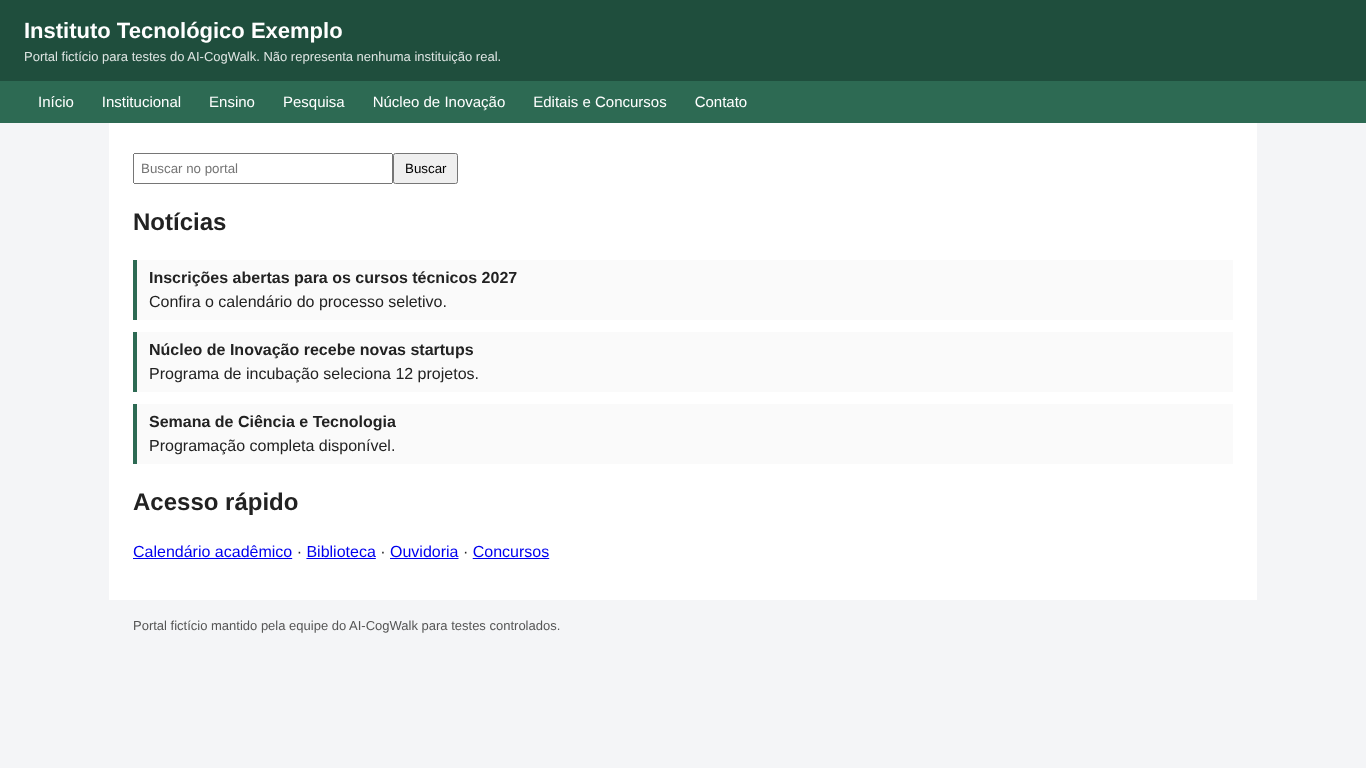
\includegraphics[width=0.78\textwidth]{figuras/captura-portal-ficticio.png}
\legend{Fonte: captura do protótipo.}
\end{figure}

\textbf{Cuidados éticos.} A navegação automatizada só faz requisições GET em páginas públicas, sem cadastro, sem formulários e com intervalo entre ações. A coleta com pessoas só começa após aprovação do Comitê de Ética em Pesquisa \cite{cns2016res510}, com consentimento, anonimização e tratamento conforme a LGPD \cite{brasil2018lgpd}.

\subsection{Cronograma}
\label{sec:cronograma}

A Figura~\ref{fig:gantt} apresenta o cronograma proposto. O Marco 2 corresponde ao método e ao \textit{benchmark}, o Marco 3 ao portal institucional e o Marco 4 às extensões e à escrita.

\begin{figure}[htb]
\centering
\caption{Cronograma proposto (meses). A barra verde já foi concluída.}
\label{fig:gantt}
\begin{ganttchart}[
  hgrid, vgrid, x unit=0.6cm, y unit chart=0.52cm,
  title label font=\scriptsize, bar label font=\scriptsize, group label font=\scriptsize\bfseries,
  bar/.append style={fill=blue!35}, group/.append style={fill=gray!60},
  milestone label font=\scriptsize\itshape
]{1}{18}
\gantttitle{2026}{2}\gantttitle{2027}{12}\gantttitle{2028}{4}\\
\gantttitlelist{11,12,1,2,3,4,5,6,7,8,9,10,11,12,1,2,3,4}{1}\\
\ganttgroup{Marco 2: método e \textit{benchmark}}{1}{4}\\
\ganttbar[bar/.append style={fill=green!50}]{Protótipo NAV, B0, piloto (feito)}{1}{1}\\
\ganttbar{Decisões em aberto e orçamento}{2}{2}\\
\ganttbar{Experimento completo com LLMs}{2}{4}\\
\ganttmilestone{Artigo do \textit{benchmark}}{5}\\
\ganttgroup{Marco 3: portal institucional}{4}{11}\\
\ganttbar{Submissão ao CEP}{4}{6}\\
\ganttbar{Capturas e previsões congeladas}{6}{7}\\
\ganttbar{Coleta com ingressantes}{8}{10}\\
\ganttbar{Análise prospectiva}{10}{11}\\
\ganttgroup{Marco 4: extensões}{11}{16}\\
\ganttbar{B2 multiagente (se justificado)}{11}{14}\\
\ganttbar{Escrita da dissertação}{13}{17}\\
\ganttmilestone{Defesa}{18}
\end{ganttchart}
\legend{Fonte: elaborada pelo autor.}
\end{figure}

\section{Considerações Finais}

A infraestrutura para responder às questões de pesquisa está construída e foi conferida de forma independente. As referências estão medidas, e a meta realista ficou clara: um bom preditor deveria chegar perto de 0,03 a 0,045 de JSD, onde está a variação natural entre amostras humanas, enquanto a \textit{baseline} semântica está em 0,29 e o acaso em 0,38. Os resultados preliminares também mostraram os limites do próprio desenho, e eles foram incorporados ao protocolo antes das rodadas principais: o critério de decisão, os intervalos, a correção para comparações múltiplas e a leitura de resultados não significativos estão definidos de antemão. O próximo passo é o experimento completo, com parâmetros congelados e orçamento aprovado; depois, o piloto prospectivo no portal do IFPB.

% =====================================================================
% ELEMENTOS PÓS-TEXTUAIS
% =====================================================================
\postextual
\renewcommand{\bibname}{Referências Bibliográficas}
\bibliography{references}

\begin{apendicesenv}
\partapendices

\chapter{Prompts (versão nav-1.1)}
\label{ap:prompts}

Este apêndice traz o texto integral dos prompts da versão \code{nav-1.1}, em inglês, como são enviados aos modelos.

\textbf{B1 (distribuição declarada), prompt do sistema:}
\begin{lstlisting}
You model how real people navigate websites. You will receive a task and the options visible on one screen.
Estimate the distribution of FIRST choices that a population of novices would make: a first-time visitor who has never used this website and does not know how its content is organized.
Do not tell which option is correct. Estimate what such people would actually click, including plausible
mistakes and minority choices. Give a probability to every option id; the probabilities must sum to 1.
\end{lstlisting}

\textbf{B1-CW: o mesmo texto, acrescido de:}
\begin{lstlisting}
Before estimating, apply the cognitive walkthrough questions that make sense before the first action,
to every option, from the novice's point of view:
Q1 (goal): would a novice with this task plausibly decide to look under this option?
Q2 (visibility): is the option noticeable on this screen, considering position, size and contrast?
Q3 (association): does the option's label connect to the task in the novice's own vocabulary?
Q4 (feedback after the action) does not apply here, because the result of the click is not visible yet.
Base the distribution on these answers.
\end{lstlisting}

\textbf{B1-R (controle): o texto do B1, acrescido de:}
\begin{lstlisting}
Before estimating, write a brief analysis of every option: in one short sentence, what a visitor would
expect to find under it and how it relates to the task.
Base the distribution on this analysis.
\end{lstlisting}

\textbf{B1-S (participante simulado), prompt do sistema:}
\begin{lstlisting}
You are a participant in a usability study: a first-time visitor who has never used this website and does not know how its content is organized.
You will receive a task and the options visible on the screen. Choose the option you would click first,
as this participant would, not as an expert. There are no right or wrong answers.
In "reason", say in one short sentence why this participant would click that option.
\end{lstlisting}

\textbf{B1-CW-S: o mesmo texto, acrescido de:}
\begin{lstlisting}
Before choosing, think briefly, as this participant, about each option: would I look here for this task (Q1)?
Do I notice it on the screen (Q2)? Does its label match the words I have in mind (Q3)? Then choose.
\end{lstlisting}

\textbf{Mensagem do usuário (exemplo real do piloto, WTC-t4; a imagem da tela segue junto):}
\begin{lstlisting}
Task: You have bet on a boxing match and would like to see the results. Where would you look for them?

The image shows the screen as the participant sees it before the first click (1366x768 pixels).
Options (id: label @ x,y,width,height):
- 0: Trending @ 125,85,95,48
- 1: Entertainment @ 220,85,133,48
- 2: Hobbies @ 353,85,91,48
- 3: Culture @ 444,85,83,48
- 4: Science @ 527,85,89,48
- 5: Society @ 616,85,85,48
- 6: Lifestyle @ 701,85,92,48
- 7: About us @ 793,85,96,48
\end{lstlisting}

\textbf{Esquemas de resposta.} B1: \code{\{distribution: [\{optionId, probability\}], rationale\}}. B1-CW: \code{\{walkthrough: [\{optionId, q1, q2, q3\}], distribution, rationale\}}, com \code{q1..q3} em \{yes, partly, no\}. B1-R: \code{\{analysis: [\{optionId, note\}], distribution, rationale\}}. B1-S: \code{\{reason, choice\}}. B1-CW-S: \code{\{walkthrough, choice\}}. Em todos, \code{optionId} e \code{choice} são restritos aos identificadores das opções.

\chapter{Como Reproduzir}
\label{ap:repro}

Este apêndice lista os comandos que reproduzem os resultados do Capítulo~\ref{cap:resultados}. Os passos 1, 2 e 4 não usam chaves de API nem fazem chamadas a LLMs.

\begin{lstlisting}
# 1. Backend e banco (PostgreSQL 16), sem chaves de API para B0/UNIFORM
cd backend && ./gradlew bootJar
java -jar build/libs/aicogwalk-backend-0.1.0.jar        # porta 8080

# 2. Importar o benchmark (revisão fixada) e rodar as referências
curl -X POST localhost:8080/api/nav/datasets/kuric2025
curl -X POST localhost:8080/api/nav/datasets/1/runs -H 'Content-Type: application/json' -d '{"method":"UNIFORM"}'
curl -X POST localhost:8080/api/nav/datasets/1/runs -H 'Content-Type: application/json' -d '{"method":"B0"}'

# 3. Piloto (requer ANTHROPIC_API_KEY e OPENAI_API_KEY)
curl -X POST localhost:8080/api/nav/datasets/1/runs -H 'Content-Type: application/json' \
  -d '{"method":"B1_CW","model":"gpt-4.1","stateKeys":["TP-t2-raiz","TP-t8-raiz","WTC-t4-raiz","WM-t8-raiz"]}'

# 4. Exportar e conferir em Python
curl localhost:8080/api/nav/runs/2/export.json > b0.json
python3 analysis/verify_b0_metrics.py <dir do modelo> b0.json uniform.json
python3 analysis/nav_kuric_analysis.py uniform.json b0.json
python3 analysis/nav_b0_crossfit.py b0.json
python3 analysis/nav_analises_complementares.py b0.json piloto-run5.json piloto-run6.json piloto-run7.json piloto-run8.json
\end{lstlisting}

Os \textit{hashes} esperados para a revisão \code{6cc9130} e os prompts \code{nav-1.1} são: UNIFORM \code{7763c4455b95e91d\ldots} e B0 \code{55de6c0fc7fe4083\ldots}. As exportações das rodadas de 13/11/2026 e a saída de cada \textit{script} estão em \code{analysis/resultados-2026-11-13/}. O código do protótipo está em \url{https://github.com/L42Matheus/ai-cogwalk}.

\end{apendicesenv}

\end{document}
